\documentclass[12pt]{article}

% Language setting
% Replace `english' with e.g. `spanish' to change the document language
\usepackage[english]{babel}

% Set page size and margins
% Replace `letterpaper' with `a4paper' for UK/EU standard size
\usepackage[letterpaper,top=1cm,bottom=1.25cm,left=1cm,right=1cm,marginparwidth=1.75cm]{geometry}

% Useful packages
\usepackage{amsmath}
\usepackage{amssymb}
\usepackage{graphicx}
\usepackage{caption}
\usepackage{subcaption}
\usepackage[colorlinks=true, allcolors=blue]{hyperref}
\usepackage{indentfirst}
%\usepackage{biblatex}
\usepackage{titling}
%\usepackage{subfig}

%Importing the library needed to support code displaying
\usepackage{listings}
\usepackage{color}
\captionsetup{font=small}

\title{A Qualitative Approach to Patch Antenna Operation}
\author{Andrey Lototskiy}
\date{\today}

\begin{document}
\maketitle

\begin{abstract}
This paper seeks to provide a qualitative explanation for the radiation mechanism, and properties of a basic rectangular patch antenna. The paper first starts by providing some motivation for why patch antennas are worth studying, before providing an overview for the rest of the structure of the paper. The paper first discusses the theoretical mechanism of how antennas radiate energy. The paper then moves into showcasing the operation of a patch antenna while simultaneously providing an explanation of how the patch antenna emits radiation. Finally, the paper closes out by pointing out some properties of patch antennas which lend them applications in certain fields.
\end{abstract}

\section{Introduction}
Among all of the antennas in use today, perhaps none is as revolutionary as the patch antenna. First envisioned in the 1950's\cite{gutton1955flat}, patch antennas were first adopted by the aerospace industry\cite{balanis2016antenna}, due to their low profile and light weight being essential for spacecraft, missiles, and airplanes. In the 1980's, with the advance of printed circuit technology, patch antennas became far cheaper to manufacture\cite{khan2015microstrip}, which brought them applications in commercial wireless communication systems.  

\begin{figure}[h]
    %\begin{subfigure}{0.5\textwidth}
    \centering
    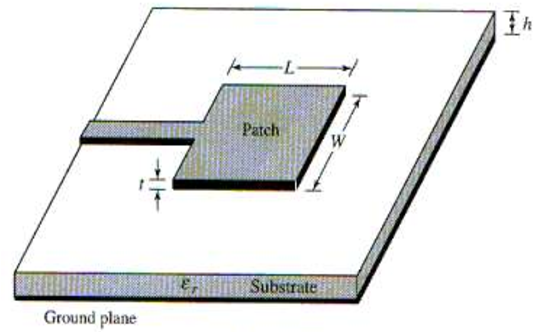
\includegraphics[width=0.5\textwidth]{patch-antenna-structure.png}
    %\end{subfigure}
    \caption{The basic structure of a patch antenna. This particular antenna is being fed with a microstrip. The ground, and the patch are conductors. The substrate is a dielectric. \cite{girase2014design}}
\end{figure}

Due to their importance, numerous theories have been created to describe and predict patch antenna operation. However, these theories are mathematically dense, and are quite challenging to comprehend. This unapproachability in theory leads to the obfuscation of how patch antennas actually work. One of the most intuitive high level ways of describing antennas is visually. While antenna simulation software does exist, it seems like nobody has used it provide a surface level introduction to patch antennas. This paper intends to do so, using the antenna simulation software HFSS. HFSS is a 3D electro-magnetic field simulator, used by RF engineers to design antennas, but it can also be used to visualize the fields in patch antennas, thereby giving an intuitive explanation of why patch antennas radiate.

This paper will first provide a theoretical overview of how antennas in general emit radiation. Next this paper will use HFSS to provide a visual explanation of the radiation mechanism of a basic patch antenna, as well as show some of its properties. None of the information presented here is particularly novel, however, the mechanism behind patch antenna operation is fascinating in its own right. 
\section{Electromagnetic Radiation}  

Before discussing patch antennas, it is important to understand how electromagnetic radiation is created in the first place. Unlike light bulbs, which generate light via the energy released by electrons decaying to lower energy levels inside atoms, antennas radiate via a completely different principle.

First, consider the electric field around some point charge, in some inertial reference frame. The electric field lines will be uniformly distributed, pointing either towards, or away from the source, depending on the charge of the source\cite{schroeder}. Next, consider a case where the charge is moving at some velocity $v_1$, and is then instantaneously accelerated to a higher velocity $v_2$. At this point, the frame of the charge has changed, and the E-field also changes.   

\begin{figure}[h]
    \begin{subfigure}{0.5\textwidth}
    \centering
    	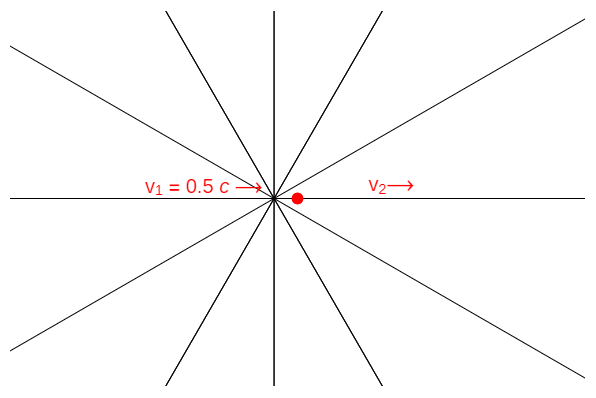
\includegraphics[width=0.9\textwidth]{charge-moving-at-v1.png}
    \end{subfigure}
    \begin{subfigure}{0.5\textwidth}
    	\centering
    	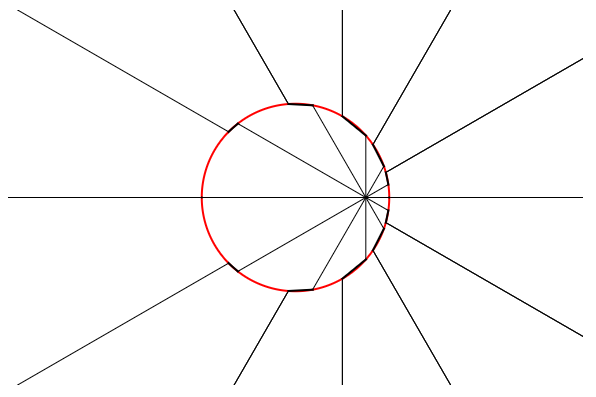
\includegraphics[width=0.9\textwidth]{charge-moving-at-v2.png}
    \end{subfigure}
    \caption{\cite{wolframwave} The electric field around a point charge at two steps in time. On the left is the electric field around a point charge moving at velocity $v_1$. On the right is the electric field around a point charge which has just instantaneous accelerated to a greater velocity $v_2$. When the charge accelerates, the new electric field lines are no longer align with the old electric field lines. }
\end{figure} 

Since the transfer of information is capped by the speed of light, the change to the E-field must also propagate at the speed of light, resulting in a region which was in the old reference frame, and a region which is in the new reference frame. The E-field lines do not align in these two regions. However, broken, or discontinuous electric field lines are not allowed, as that would violate Gauss's law. As a result, the electric field lines must connect from the frame where the velocity of the charge was $v_1$ to the frame with velocity $v_2$ \cite{schroeder}. There is therefore a bend, or kink in the electric field, which propagates to infinity at the speed of light \cite{schroeder}. In this example, the charge accelerated instantaneously from one velocity to the next. This obviously does not happen in reality, but the principle for the bending of the electric field still holds.

Now consider the electric field created by two opposite charges. The E-field points from the positive to the negative charge as shown in figure 3. 
\newpage
\begin{figure}[h]
    %\begin{subfigure}{0.5\textwidth}
    \centering
    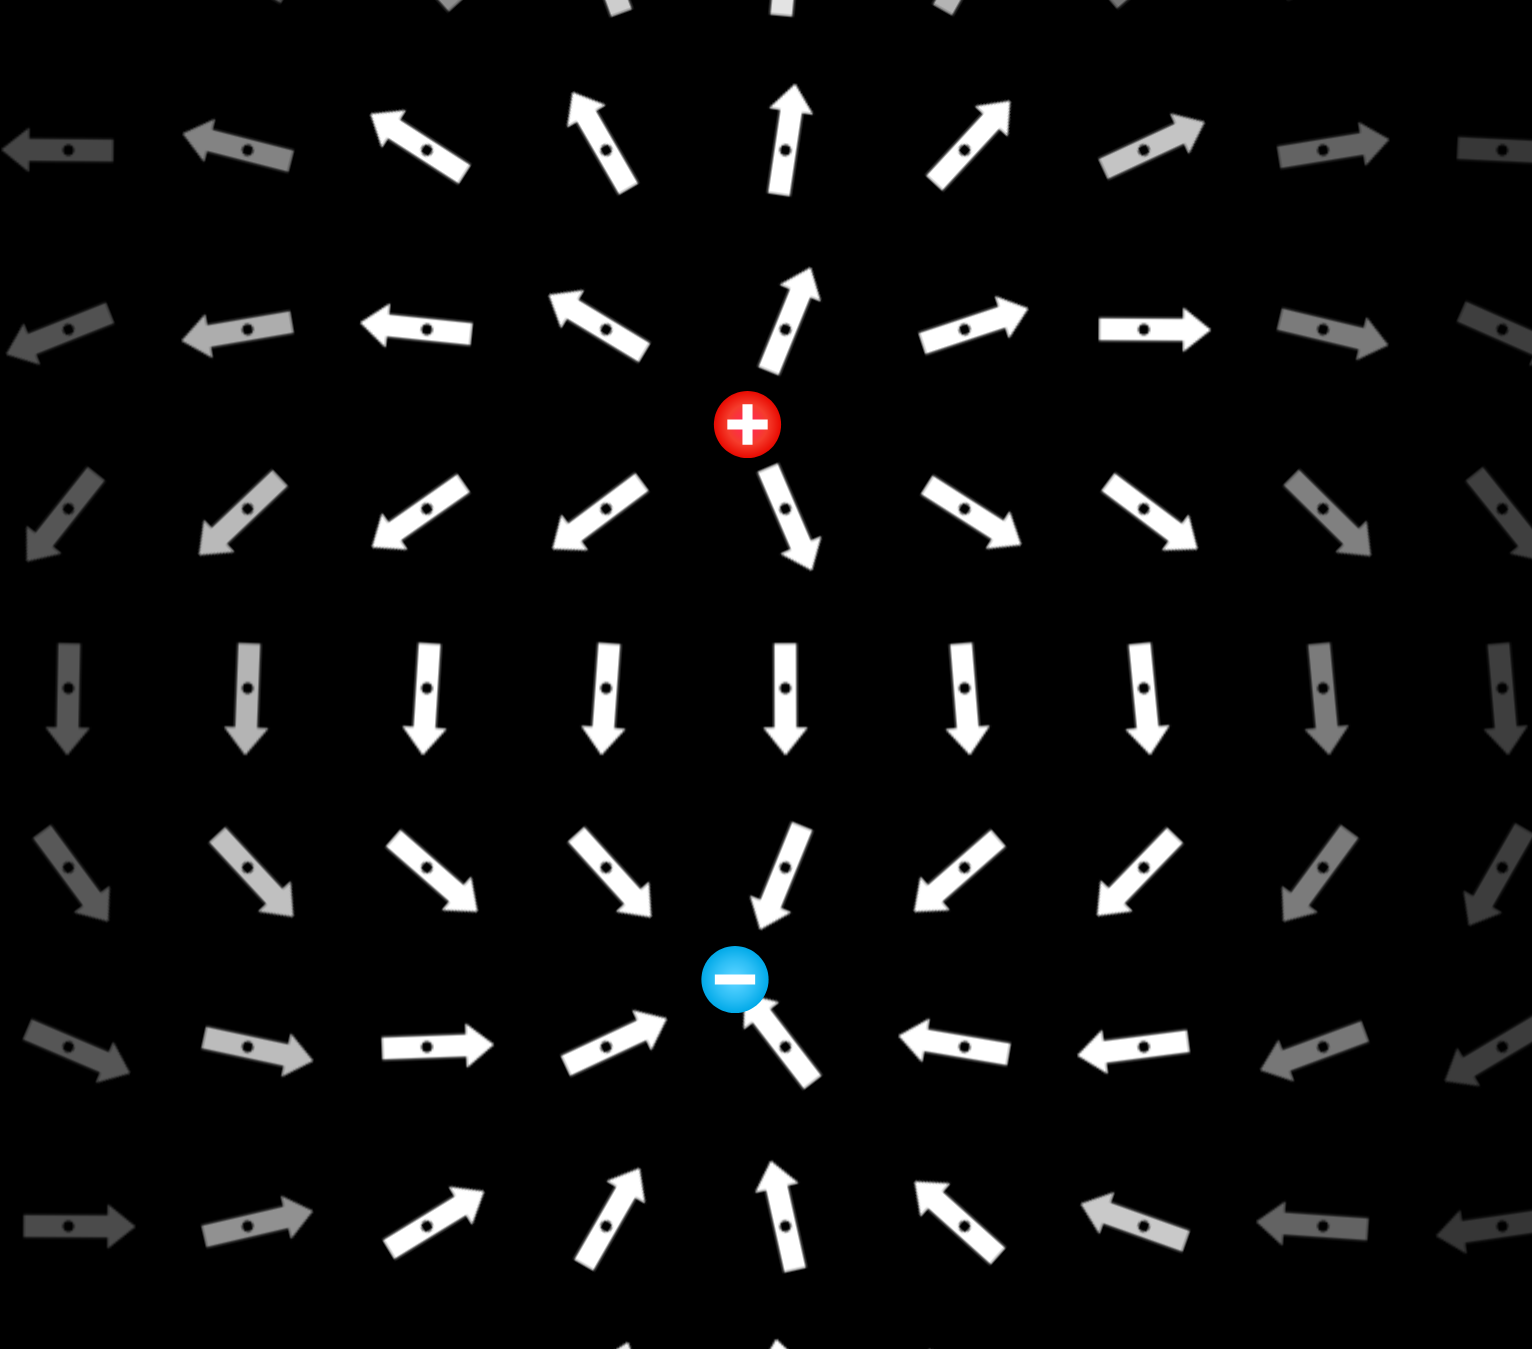
\includegraphics[width=0.3\textwidth]{positive-negative-EField.png}
    %\end{subfigure}
    \caption{The electric field around two point charges of equal magnitude, but of opposite sign.}
\end{figure} 

For the sake of simplicity, only consider one electric field line. Next, suppose that the two charges are oscillating towards each other, as shown in figure 4. The charges are moving sinusoidally (simple harmonic motion), so they are constantly experiencing an acceleration. Initially, the E-field points from the positive charge to the negative charge. As the two charges accelerate towards each other, the E-field starts to kink due to the changing reference frame of the two charges. When the two charges are very close to each other, the E-field is negligible, since the signs of the charges cancel. However, the previous E-field is still propagating outwards, and so the ends of the field lines, which started and ended on the charges, join together to create a closed loop. This loop is the radiation emitted.

\begin{figure}[h]
    \centering
    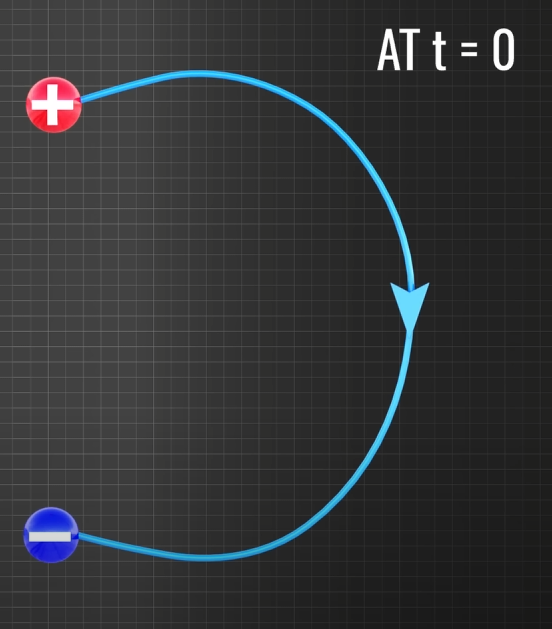
\includegraphics[width=0.20\textwidth]{dipole-at-t0.png} 
    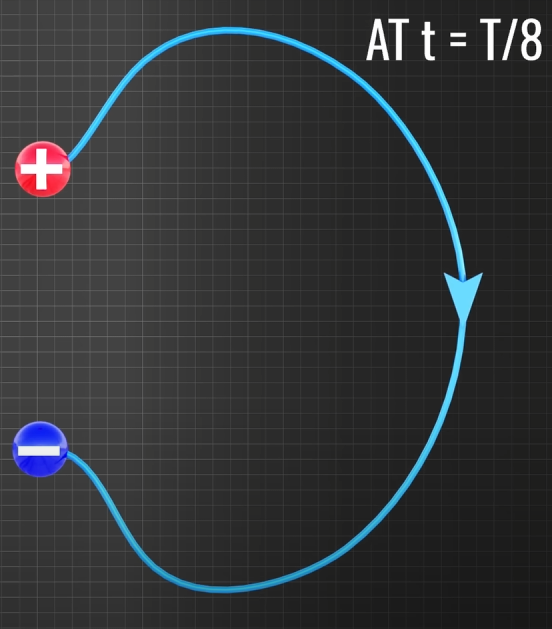
\includegraphics[width=0.20\textwidth]{dipole-at-t1.png}
    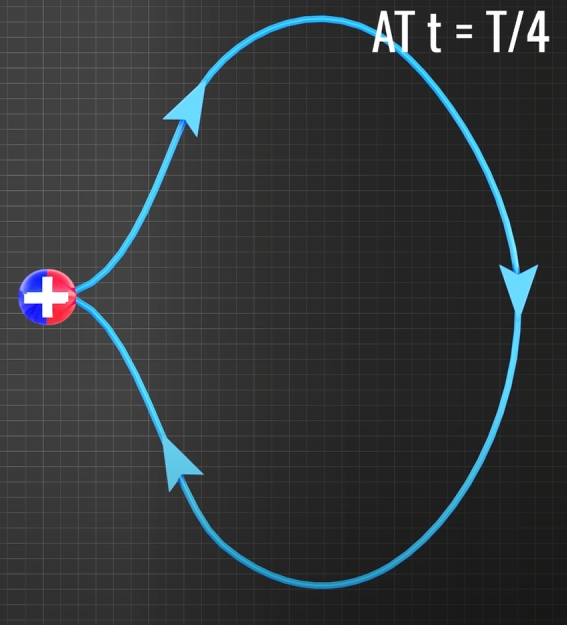
\includegraphics[width=0.20\textwidth]{dipole-at-t2.png}
    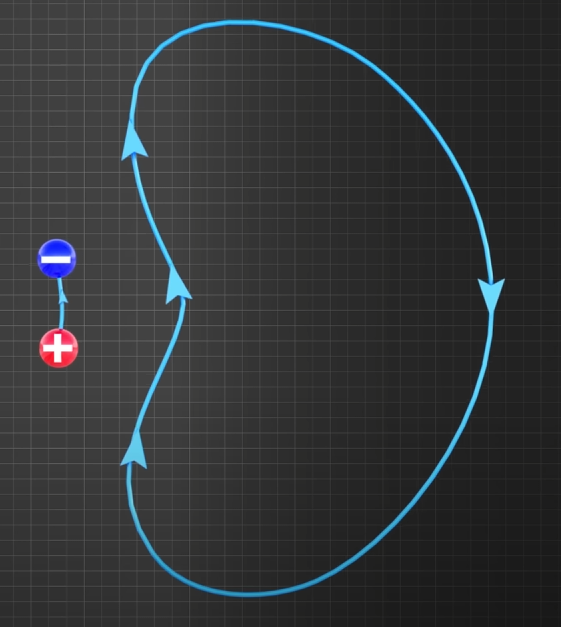
\includegraphics[width=0.20\textwidth]{dipole-at-t3.png}
    \caption{The creation of an electromagnetic wave via the oscillation of a positive and negative charge. Note that this is just the electric portion of the wave. The magnetic portion of the wave is not shown here.\cite{lesic}}
\end{figure}

It is important to remember that there is also a magnetic field, which is perpendicular to the electric field. For simplicity, the magnetic field is omitted in this paper. It also may be tempting consider the closed E-field loop as one complete wave. However, observe that the charges have not fully returned to their starting positions, and therefore have not yet completed a full oscillation. For this reason, the one closed field loop shown in figure 4 is actually half of the emitted signal, and the other half will be generated when the charges oscillate back to their original positions. It follows that the wavelength of the radiation emitted is equal to the length between two electric field wave fronts, oriented in the same direction. As such, the rightmost image in figure 4 has one half the wavelength of the radiation emitted by the charges.

\section{Patch Antenna Characteristics and radiation Mechanisms}

As shown in figure 1, a basic patch antenna consists of a very thin metallic strip (the patch), placed a small fraction of a wavelength above a metallic ground plane. In between the patch, and ground plane, is a dielectric. Dielectrics are electronic insulators which can be polarized by an external electric field. The three most popular models used to describe patch antennas are, the transmission line model, the cavity model, and the full wave model\cite{balanis2016antenna}. Since the transmission line model gives the best visual insight\cite{balanis2016antenna} into patch antenna operation, this model will be used. It should be noted however, that the transmission line model is only valid for rectangular patch antennas, and doesn't give the most accurate results\cite{balanis2016antenna}.  

\section{E-Field on the Patch}
It is important to recognize that electronically, a patch antenna is very similar to a capacitor. As a result, certain common properties of capacitors apply with patch antennas. For one, the E-field between the ground plane and the patch should be uniform, due to the fact that the electric field between two plates of opposite and equal charge is uniform. Furthermore, since the patch and ground plane are of finite size, the edges of the patch undergo fringing.
\begin{figure}[h]
    %\begin{subfigure}{0.5\textwidth}
    \centering
    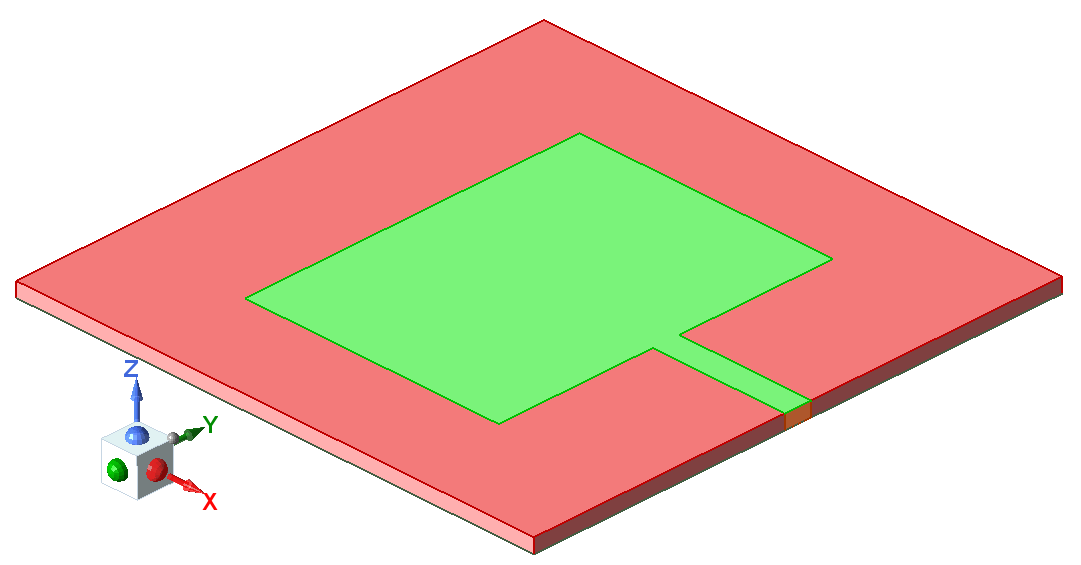
\includegraphics[width=0.5\textwidth]{2.4GHz-basic-pa.png}
    %\end{subfigure}
    \caption{A basic PA designed in HFSS to radiate at 2.4 GHz. The green material on top is the patch, with the red material being the substrate. The substrate has a relative permittivity of 4.4. There is a ground plane beneath the substrate, although it is not visible here. The patch itself is 29.4 mm long in the x direction, and 38 mm long in the y direction. The thickness of the patch and ground plane is negligible with respect to the substrate thickness. }
\end{figure}

Figure 6 depicts the aforementioned fringing in the patch antenna. The strong E-field on the edge of the patch is from fringing. However, the midpoint along the length of the patch has no fringing, implying that the E-field there is zero.

\begin{figure}[h]
    %\begin{subfigure}{0.5\textwidth}
    \centering
    \includegraphics[width=0.5\textwidth]{basic-patch-antenna-MagE-on-patch.png}
    %\end{subfigure}
    \caption{This depicts the same PA from figure 3, with an RF current applied to the patch. The magnitude of the E-field is being shown on the top side of the patch.}
\end{figure}

To gain further insight, consider the direction of the E-field at the various points on the top surface of the patch. As shown in figure 7, at either ends of the patch, the E-field is the strongest, however, the E-fields at the ends of the patch point in opposite vertical directions, and in the same horizontal directions. The reason as to why this happens is because the patch antenna is being supplied with alternating current (AC), not direct current (DC). AC behaves differently with capacitors than DC. For one, AC can flow through a capacitor, which explains why current is flowing through the antenna in the first place. However, the AC current does not flow smoothly through the capacitor. Because of the disconnect in the circuit, there is a change in medium in between the patch and ground plane. The technical term for this is an impedance mismatch. As a result of the impedance mismatch, some of the current is reflected back into the patch, rather than going through the ground plane to complete the circuit. 

\begin{figure}[h]
    %\begin{subfigure}{0.5\textwidth}
    \centering
    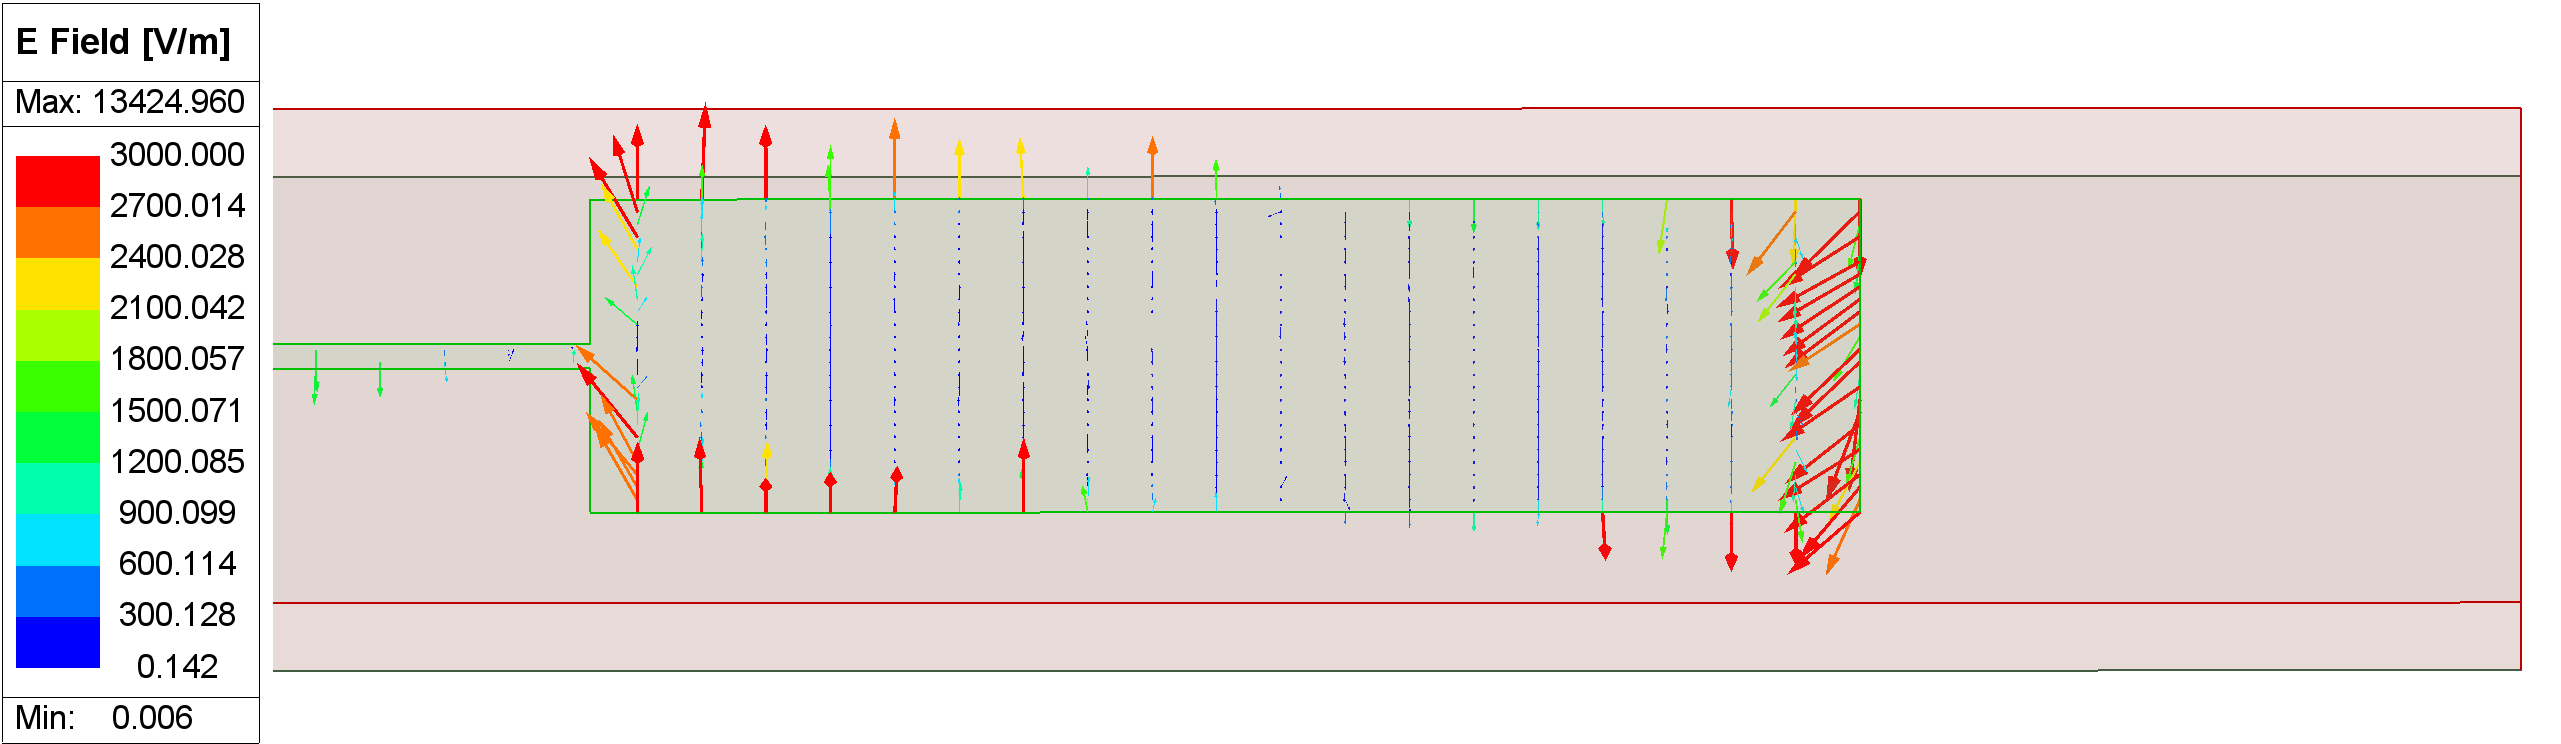
\includegraphics[width=0.5\textwidth]{E-field-onPatch-t0.png}
    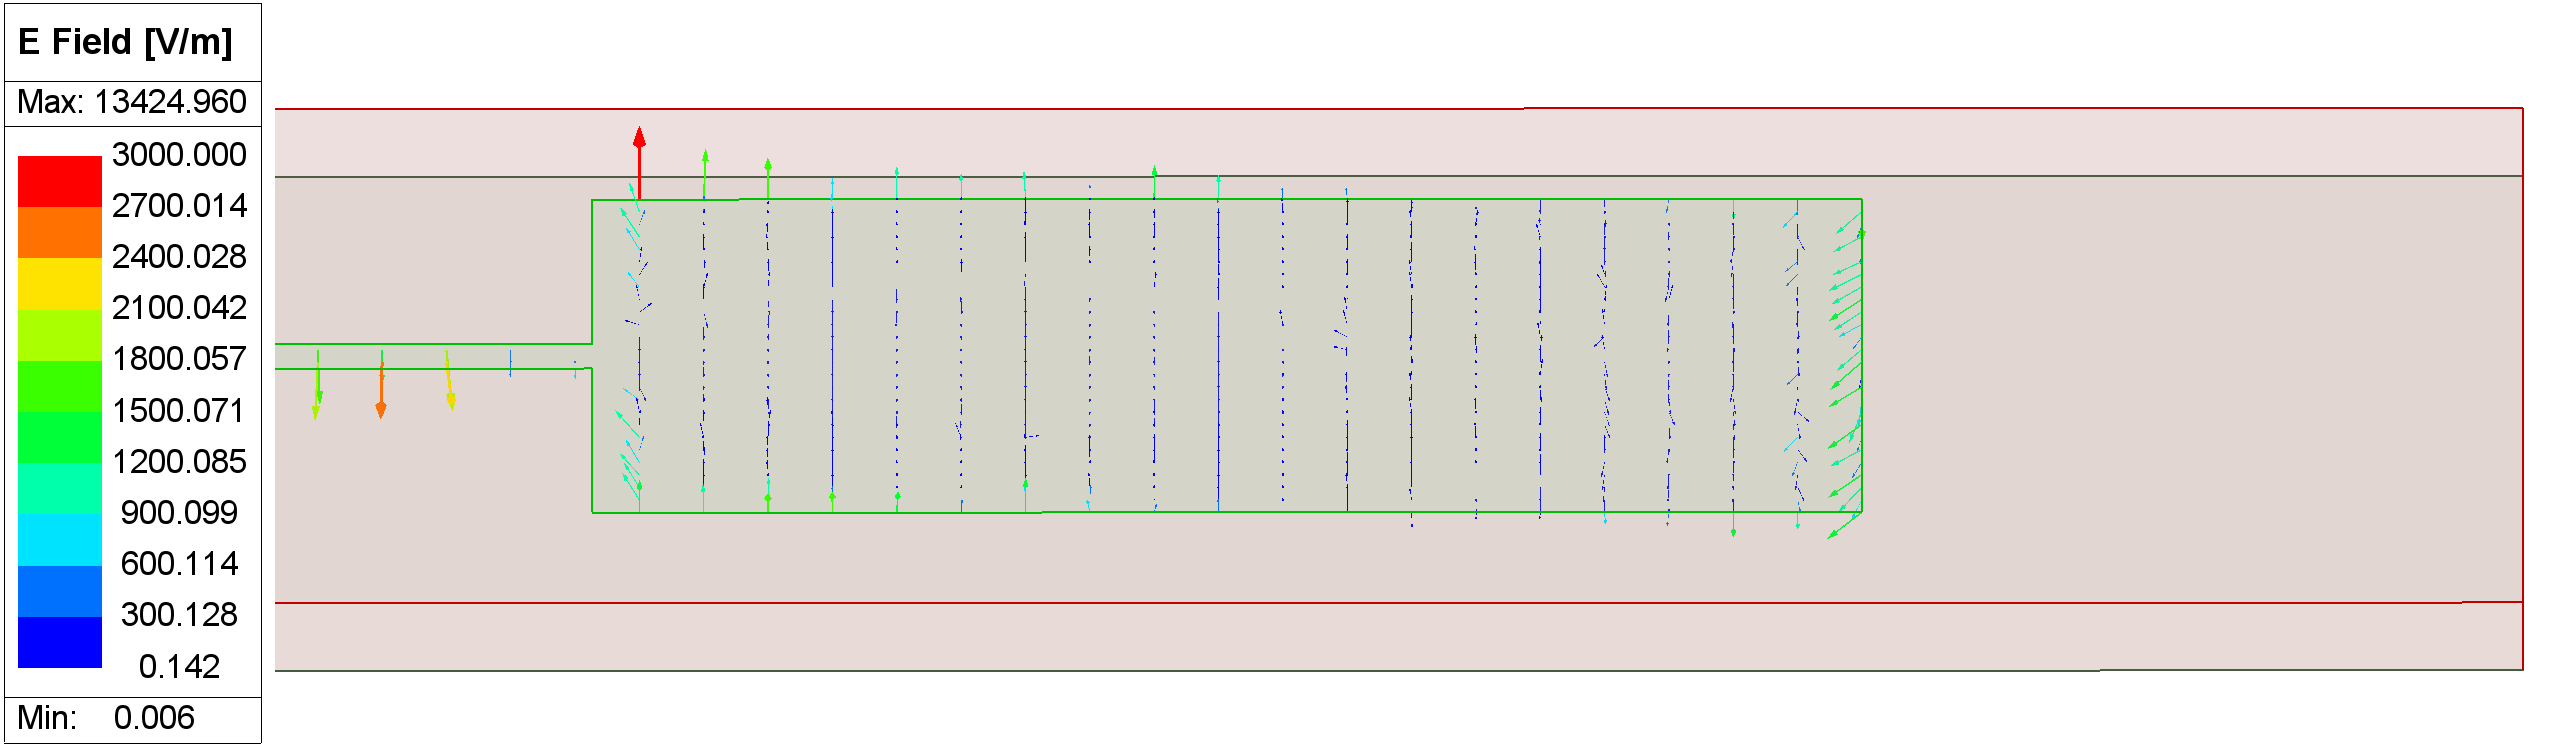
\includegraphics[width=0.5\textwidth]{E-field-onPatch-t1.png}
    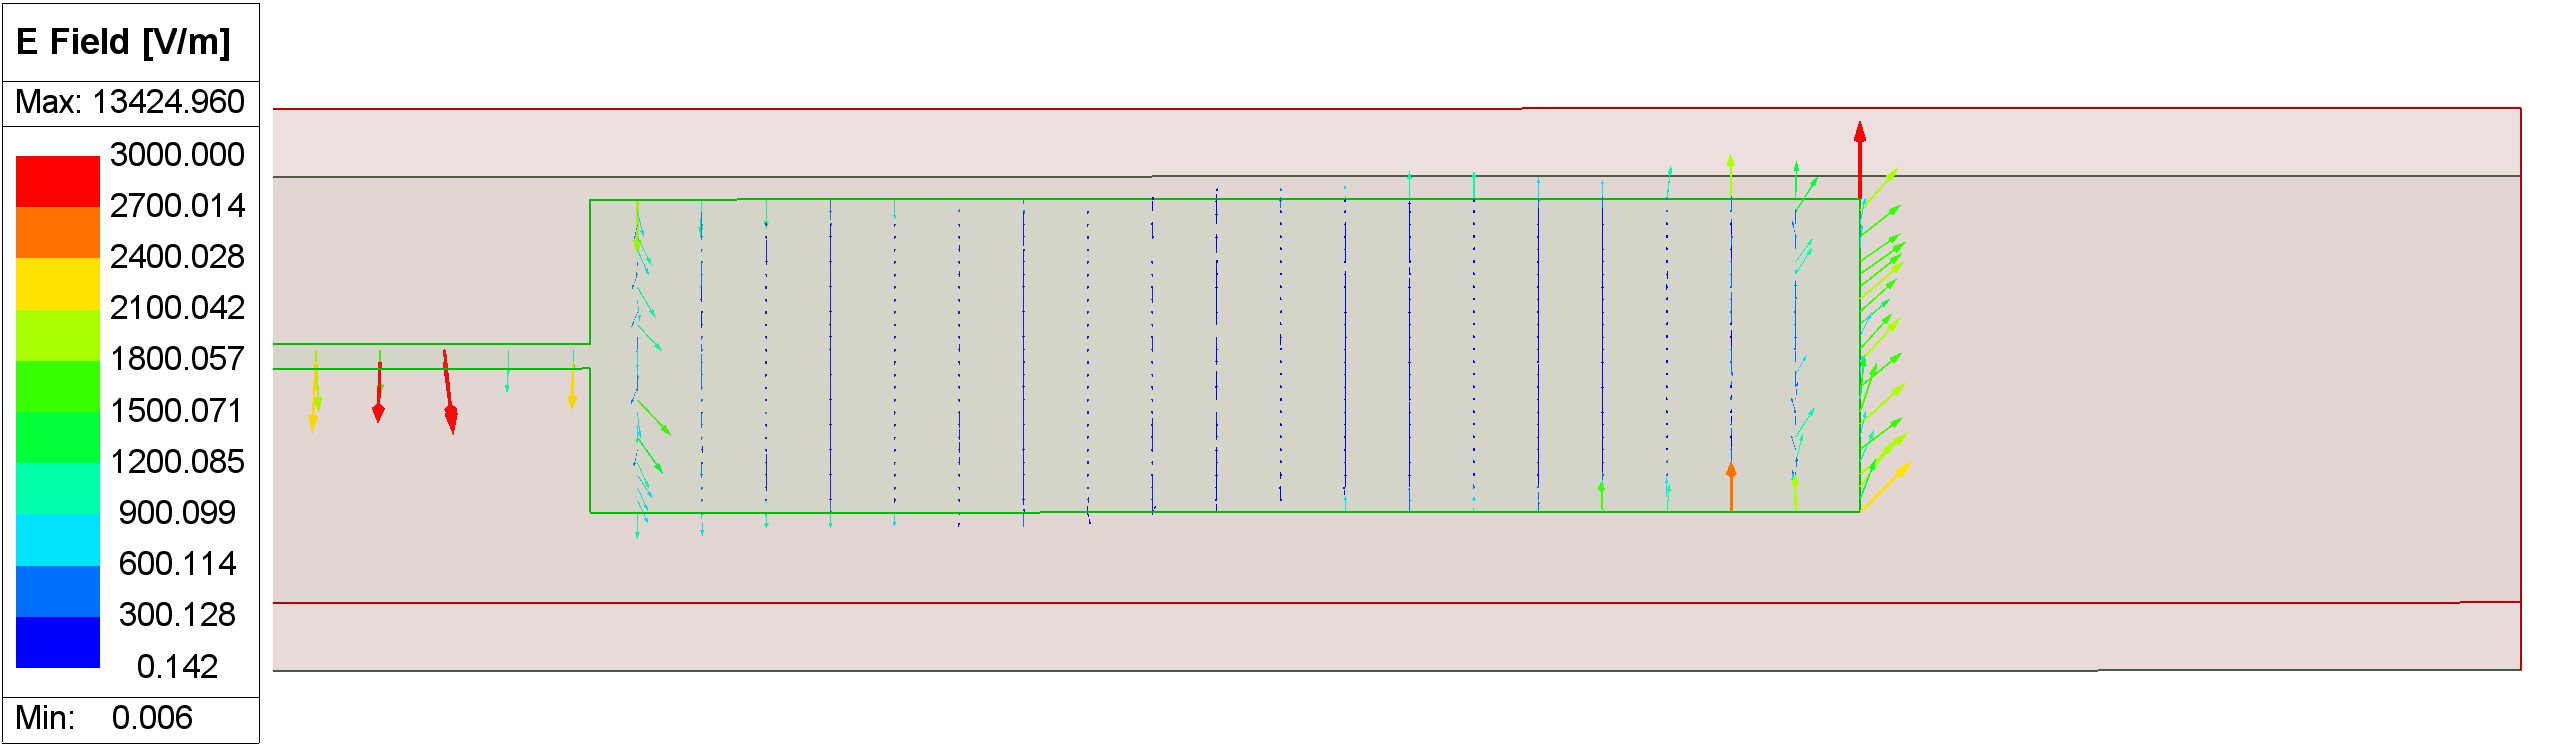
\includegraphics[width=0.5\textwidth]{E-field-onPatch-t2.png}
    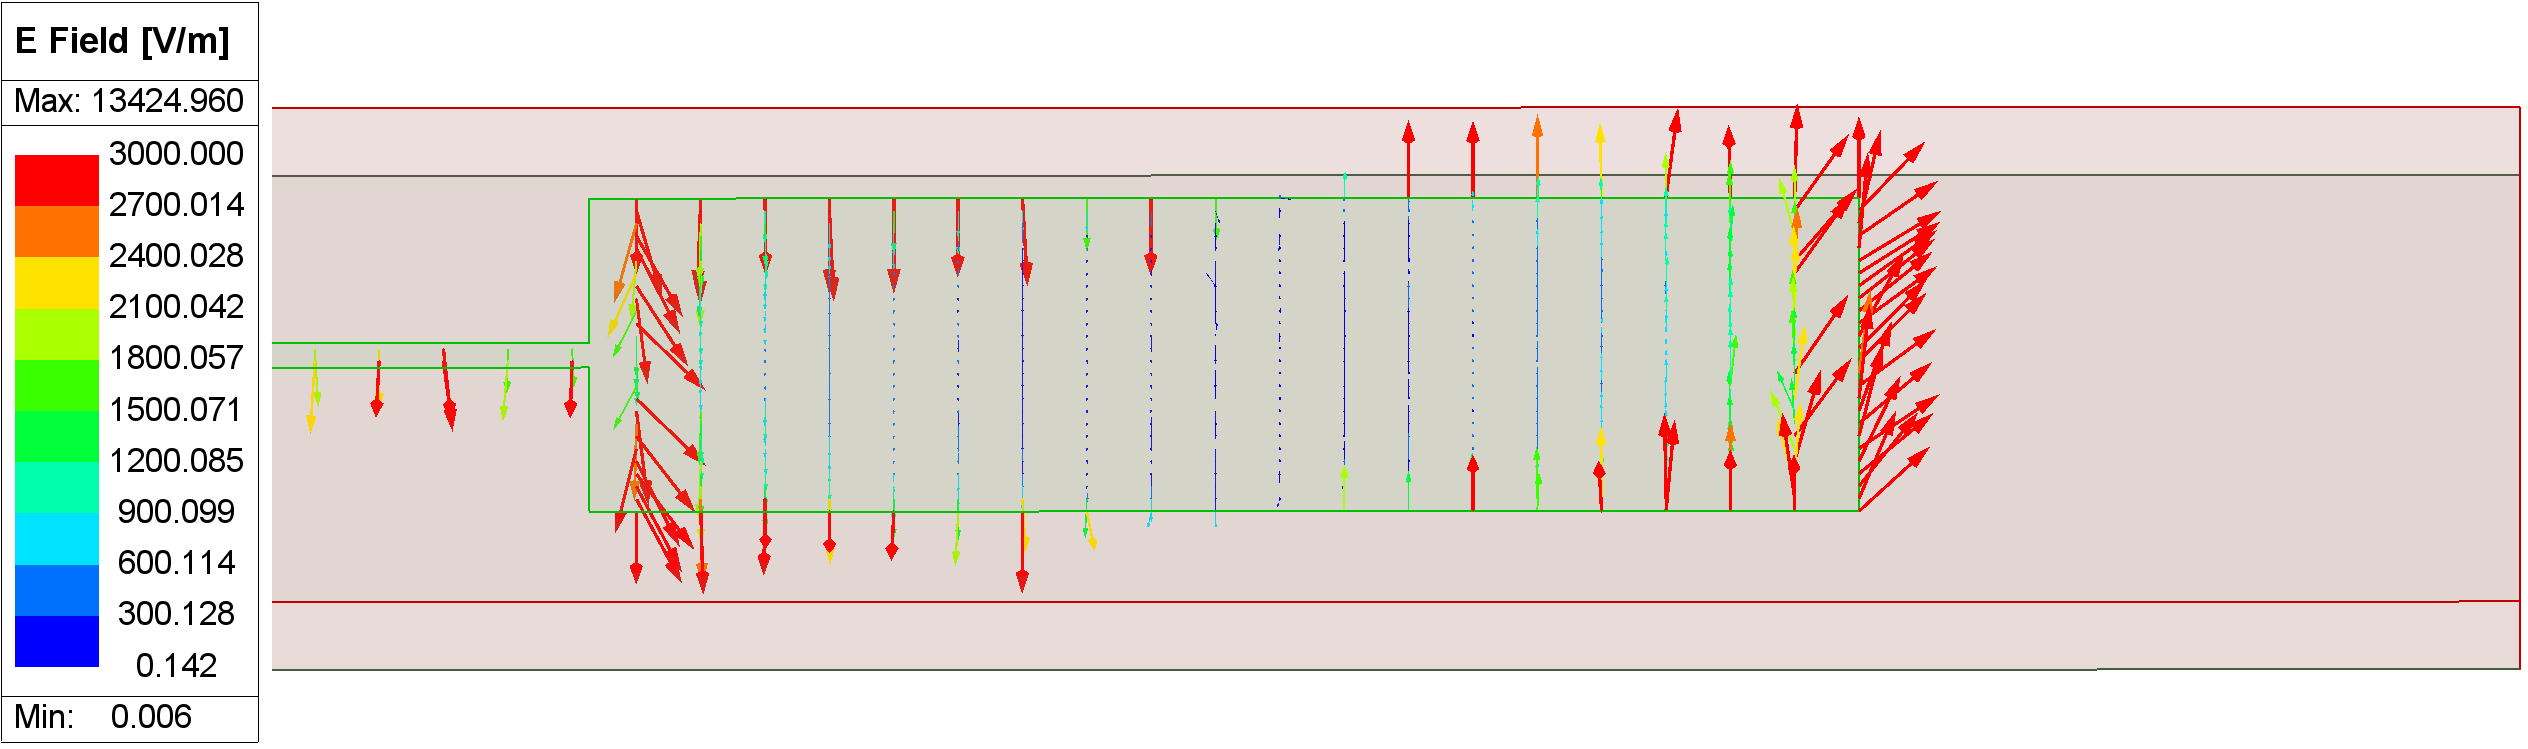
\includegraphics[width=0.5\textwidth]{E-field-onPatch-t3.png}
    %\end{subfigure}
    \caption{This shows the E-field as a vector on the patch. Subsequent images show how the E-field changes on the patch with time. The chronological ordering of the images is top to bottom (higher images are earlier in time).}
\end{figure}

The result of this reflected current is that the E-field forms a standing wave between the patch and the ground plane. This standing wave is apparent in figure 7, where the E-field can clearly be seen oscillating back and forth, but not moving forwards, as would be expected for a traveling wave. The oscillating E-field, combined with the fringing effects leads to the formation of E-M radiation.

\section{Near Field Radiation}

The immediate effect on the electric field near the patch itself is that it results in the creation of an electric dipole. Since the standing wave is constantly oscillating, the patch is constantly flipping between which side of it is positively and negatively charged, as shown in figure 8. The end result, is that near the patch, the E-field matches the E-field presented in the hypothetical model of antenna radiation. A key consideration to make is that since the ground plane is larger than the patch itself, the dipole is functionally cut in half, meaning that it only radiates in one direction. Figure 8 shows this, because the E-field on the underside of the antenna is negligible.

\newpage
\begin{figure}[ht]
    %\begin{subfigure}{0.5\textwidth}
    \centering
    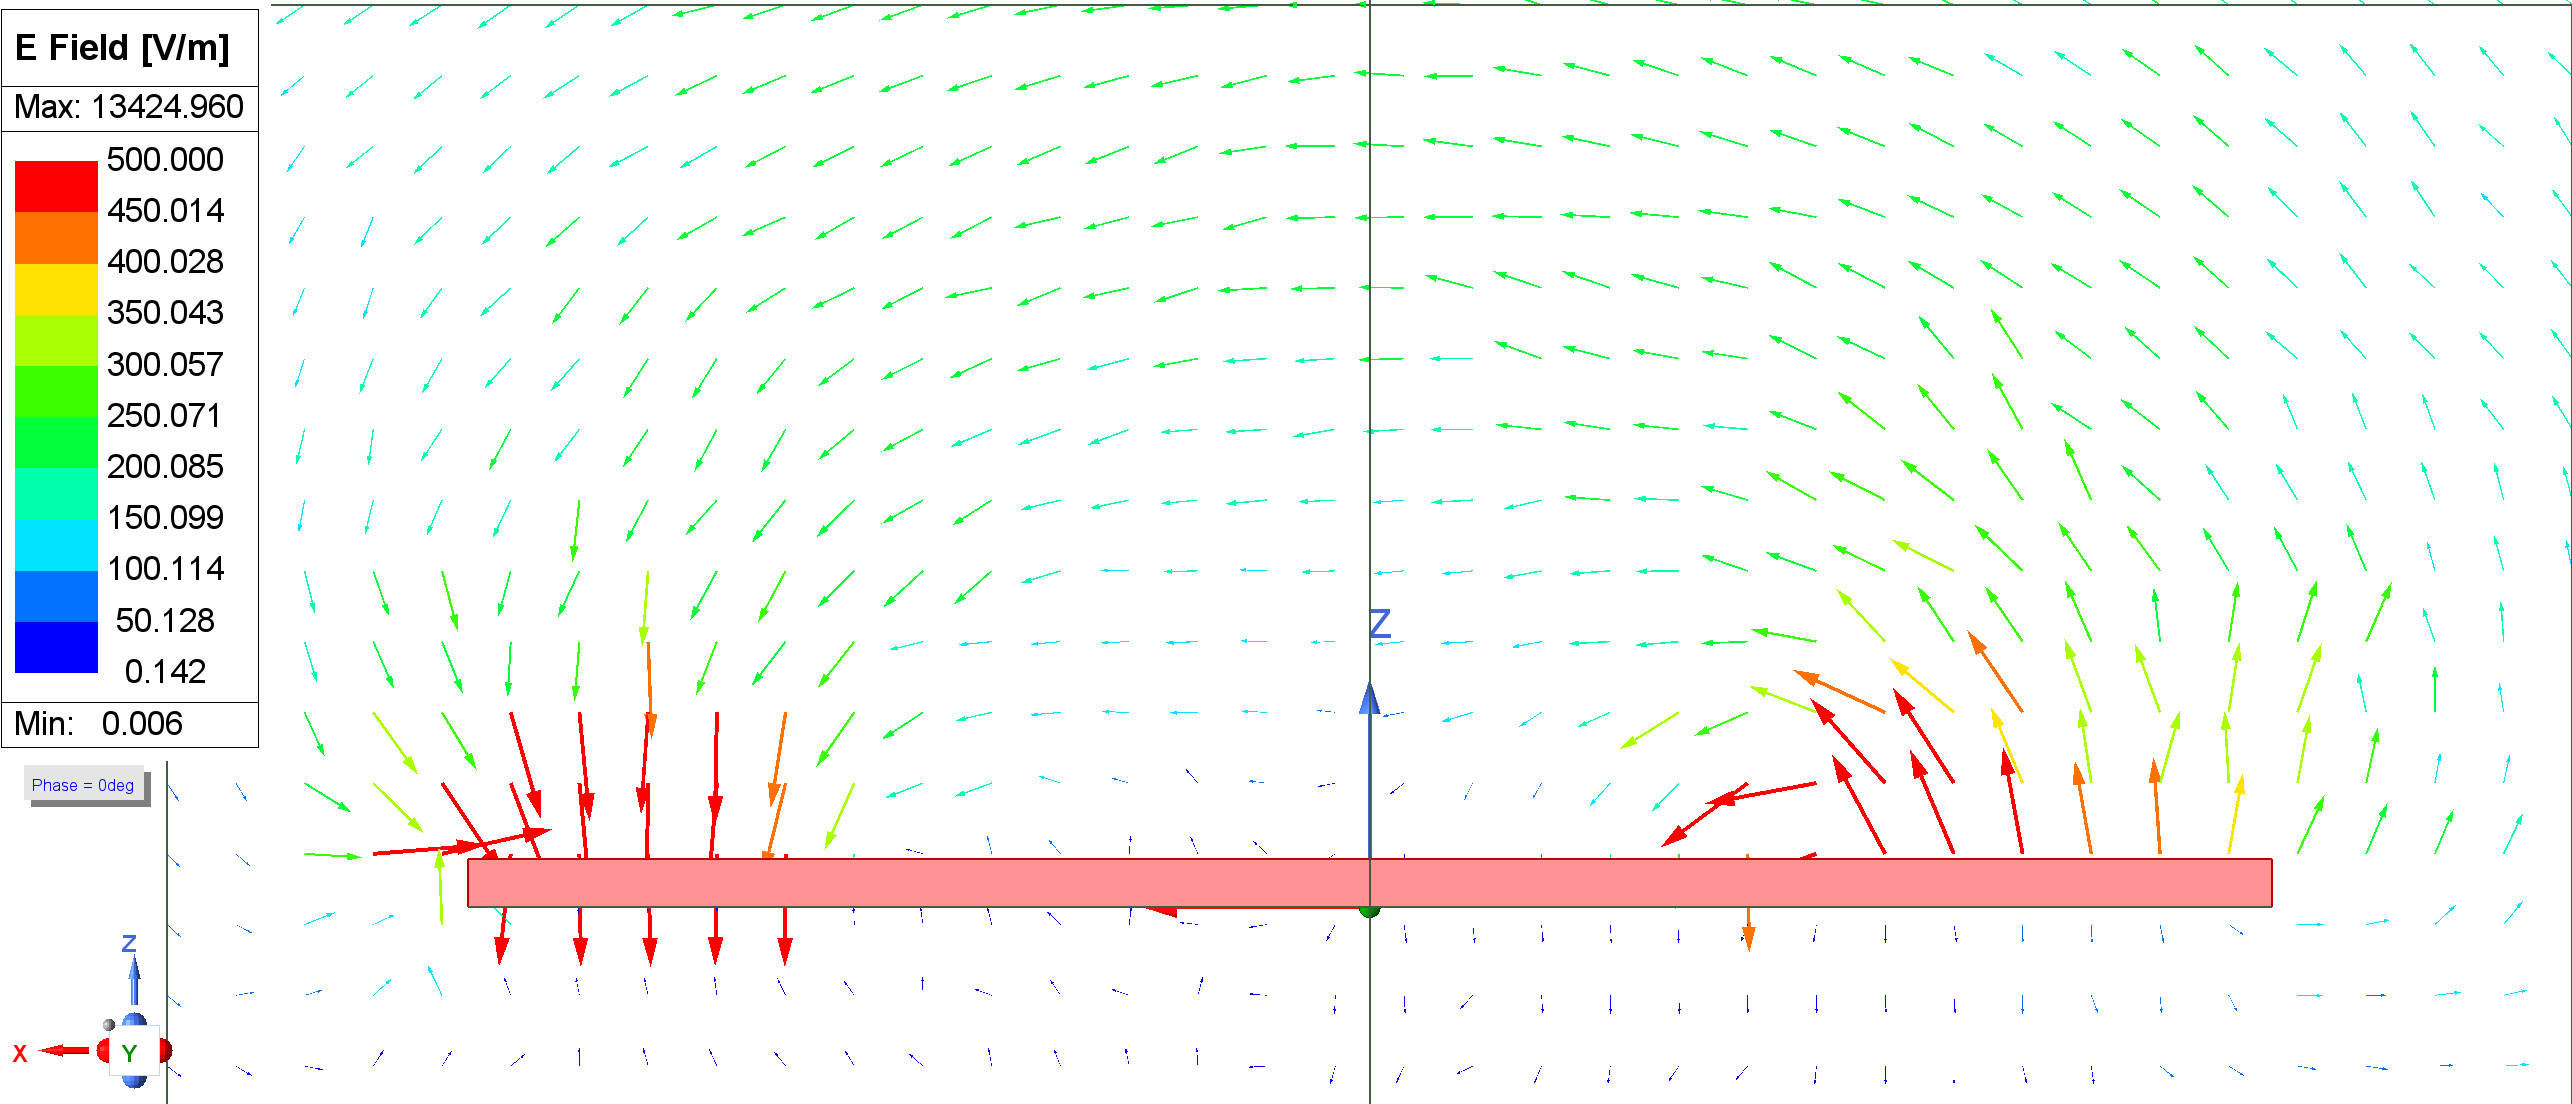
\includegraphics[width=0.5\textwidth]{patch-antenna-NearEfield-t0.png}
    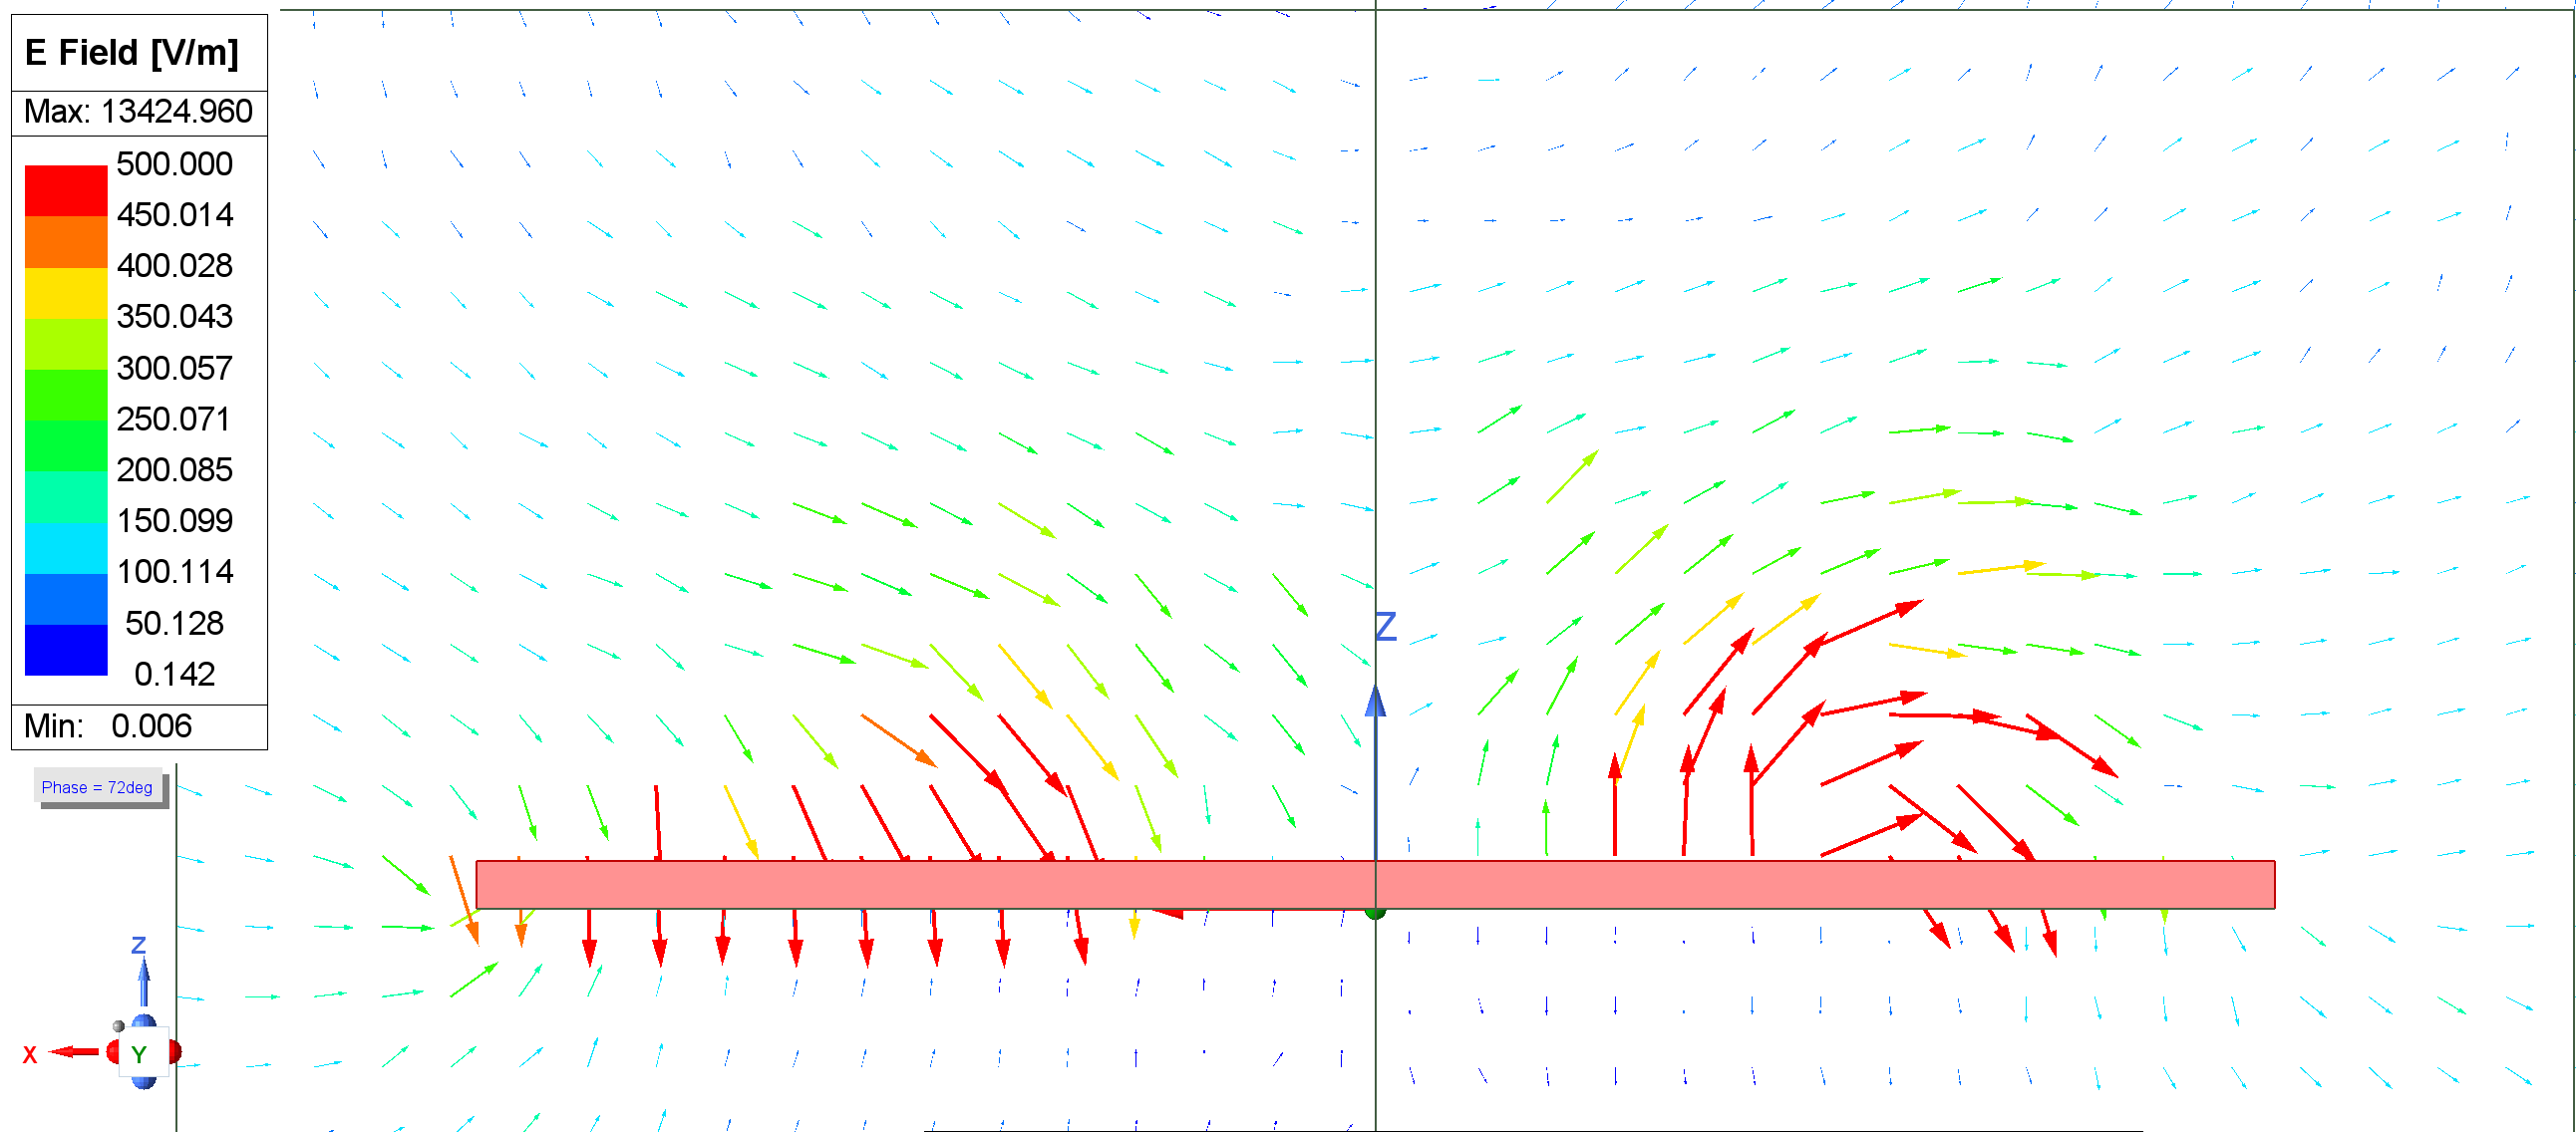
\includegraphics[width=0.5\textwidth]{patch-antenna-NearEfield-t1.png}
    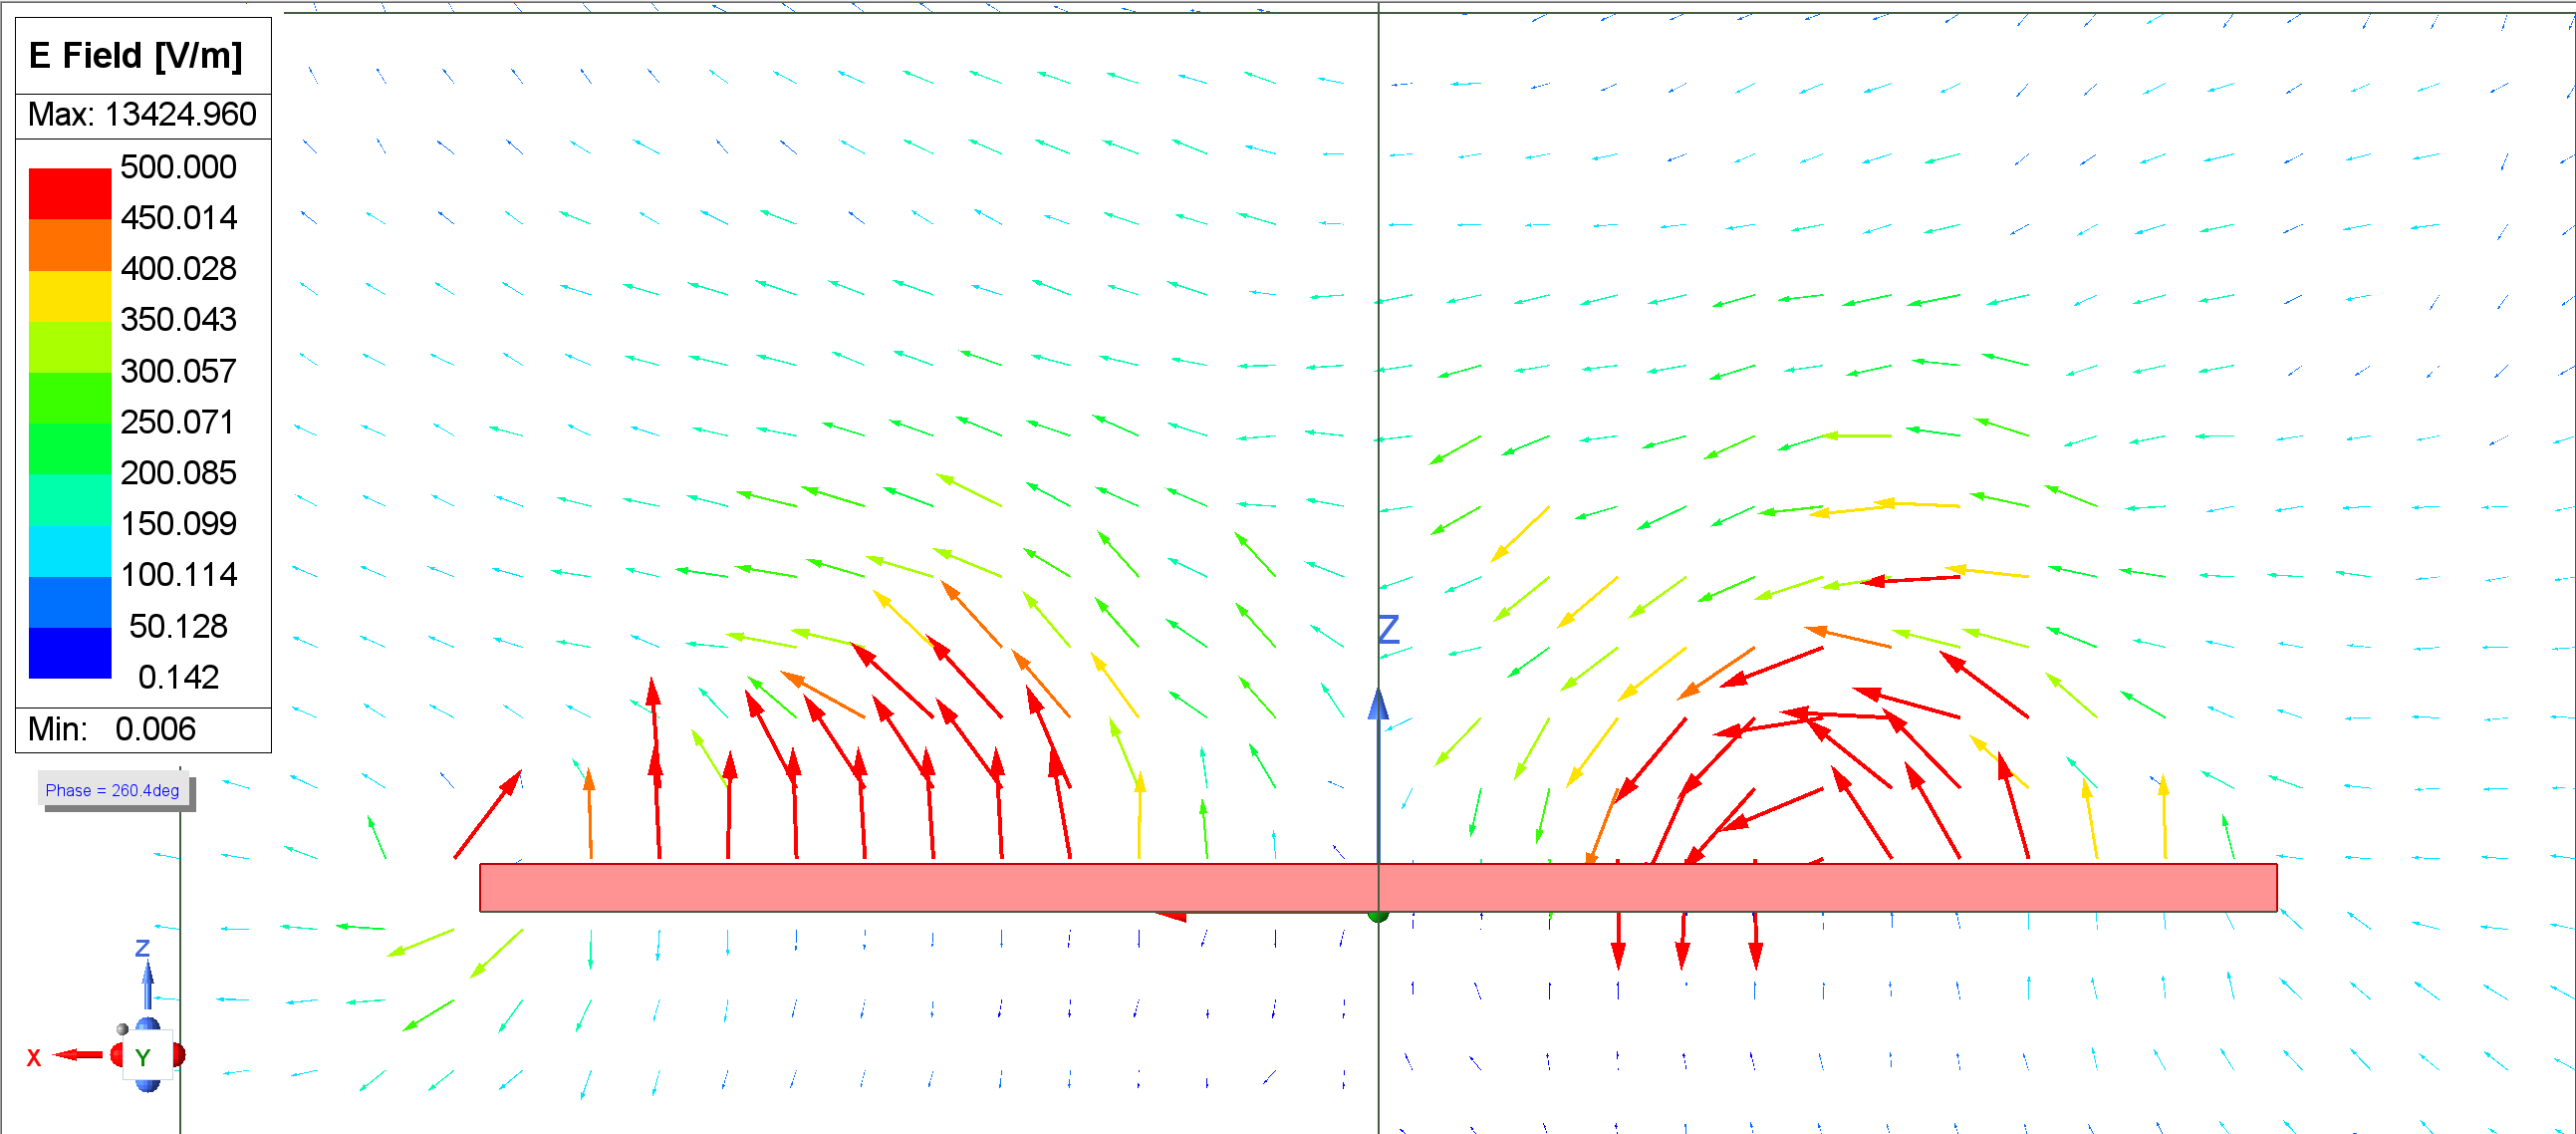
\includegraphics[width=0.5\textwidth]{patch-antenna-NearEfield-t2.png}
    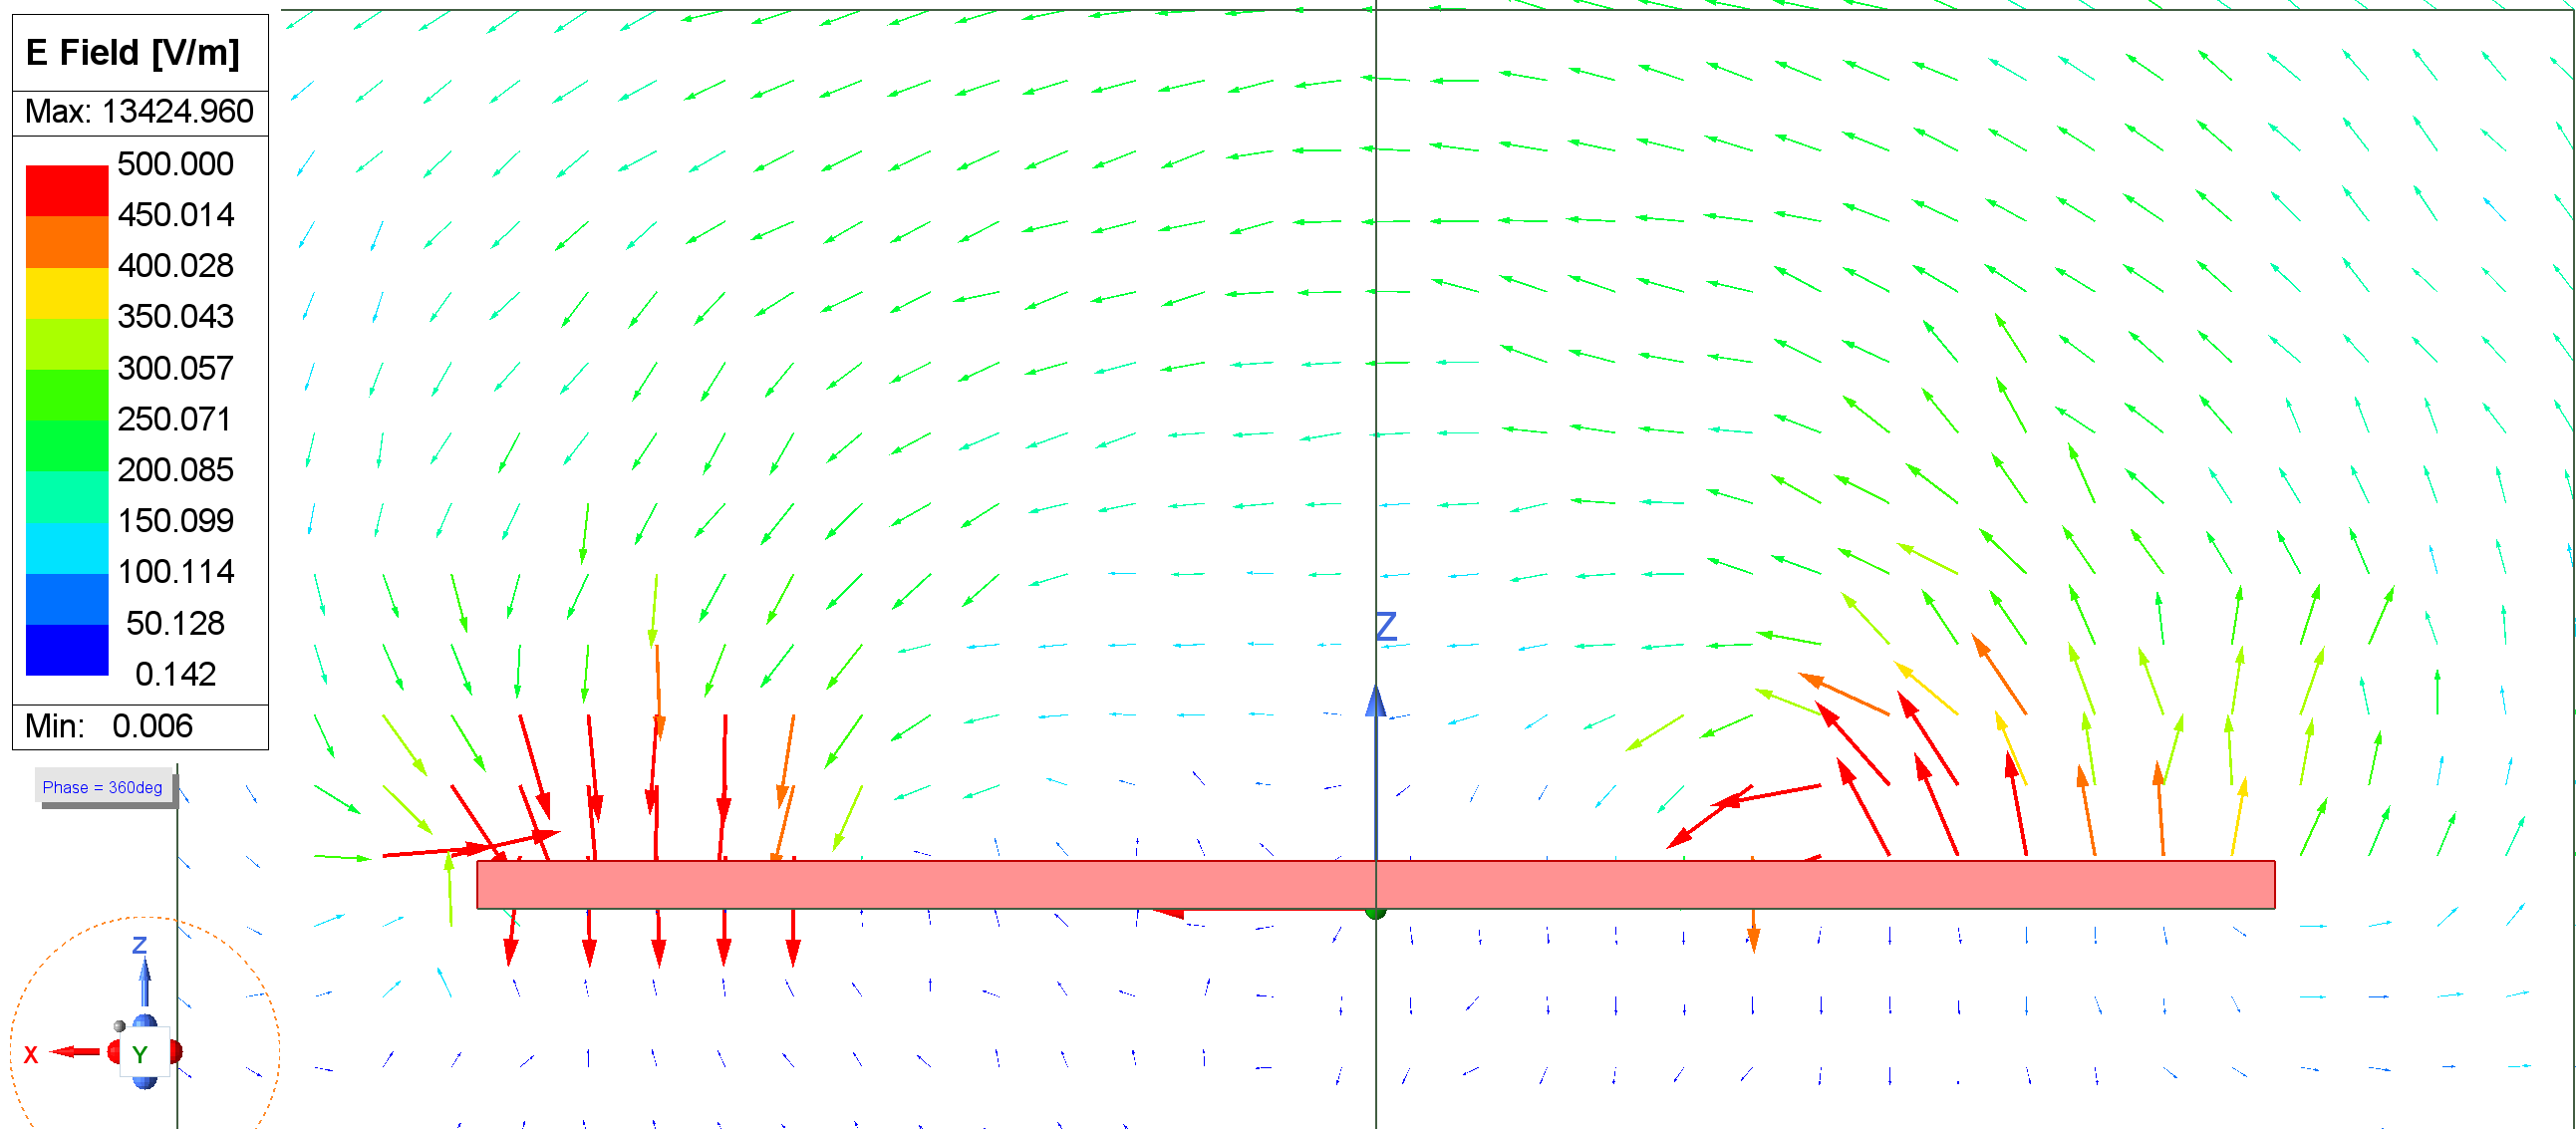
\includegraphics[width=0.5\textwidth]{patch-antenna-NearEfield-t3.png}
    %\end{subfigure}
    \caption{This shows the E-field near the patch, at snapshots in time. Observe that at a certain distance the E-field appears to travel from one point of high E-field strength to the other. In other words, from a certain distance the overall pattern of the E-field matches the expected pattern of an E-field formed by a positive and negative pair of charges.}
\end{figure}  



\section{Far Field Radiation}

The dipole created near the patch propagates outwards, just like the dipole propagates in section 2. As mentioned in the previous section, radiation only occurs broadside to the patch, due to the ground plane being larger than the patch. Furthermore the radiated E-field is parallel to the ZX plane, as is evident from figures 7, 8, and 9. 

\begin{figure}[h]
    \centering
    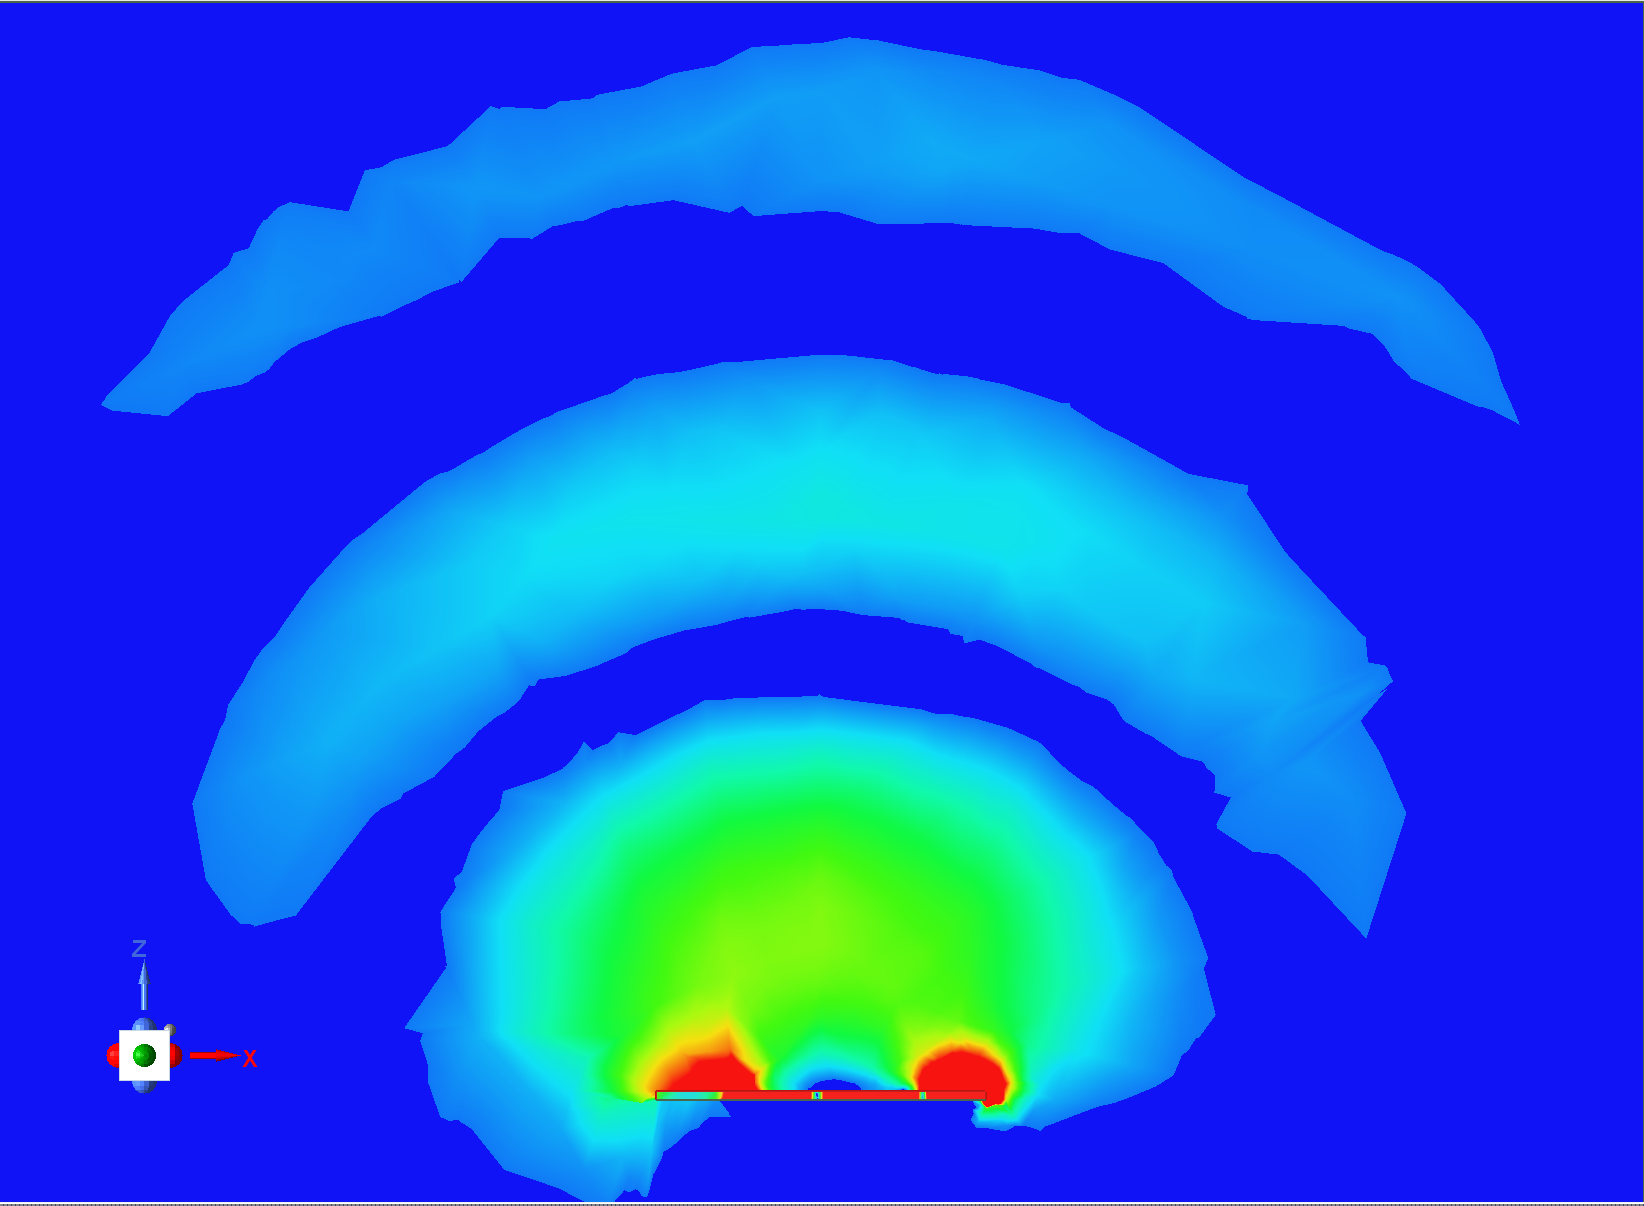
\includegraphics[width=0.35\textwidth]{basic-patch-antenna-radiating-t0.png} 
    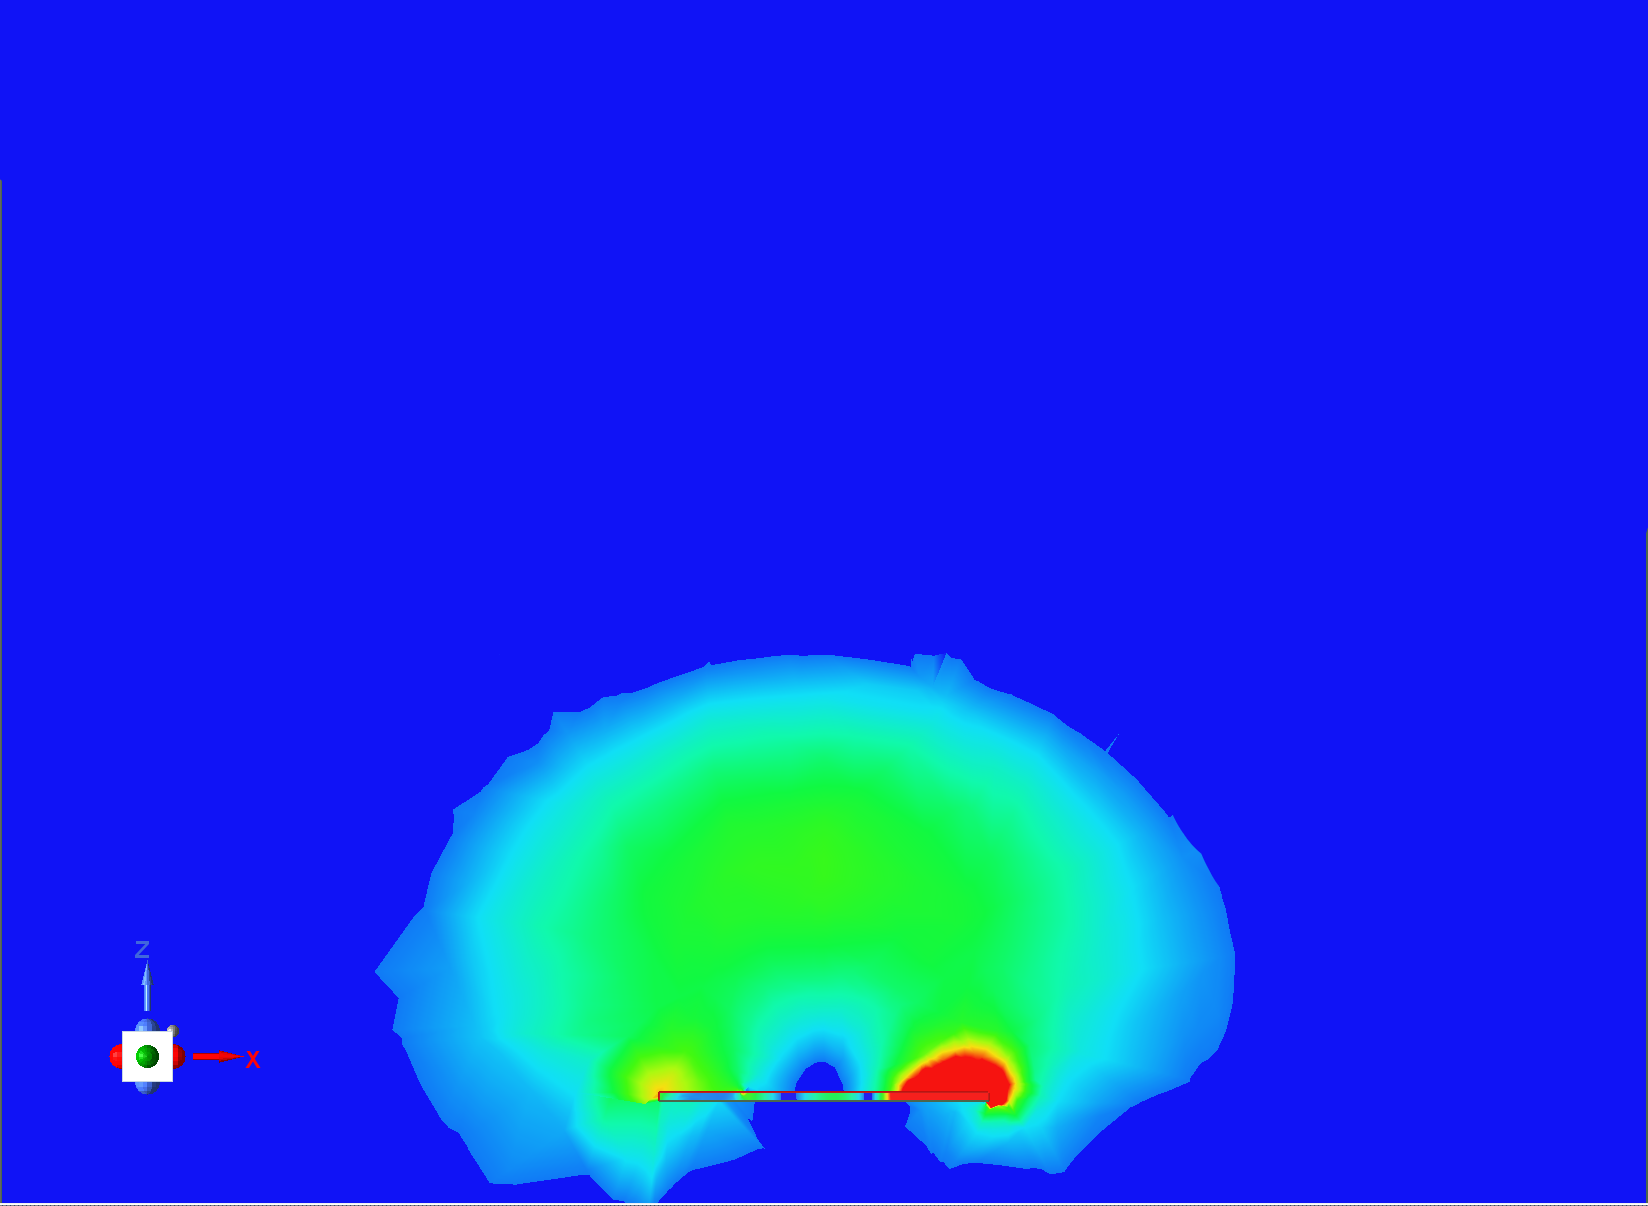
\includegraphics[width=0.35\textwidth]{basic-patch-antenna-radiating-t1.png}
    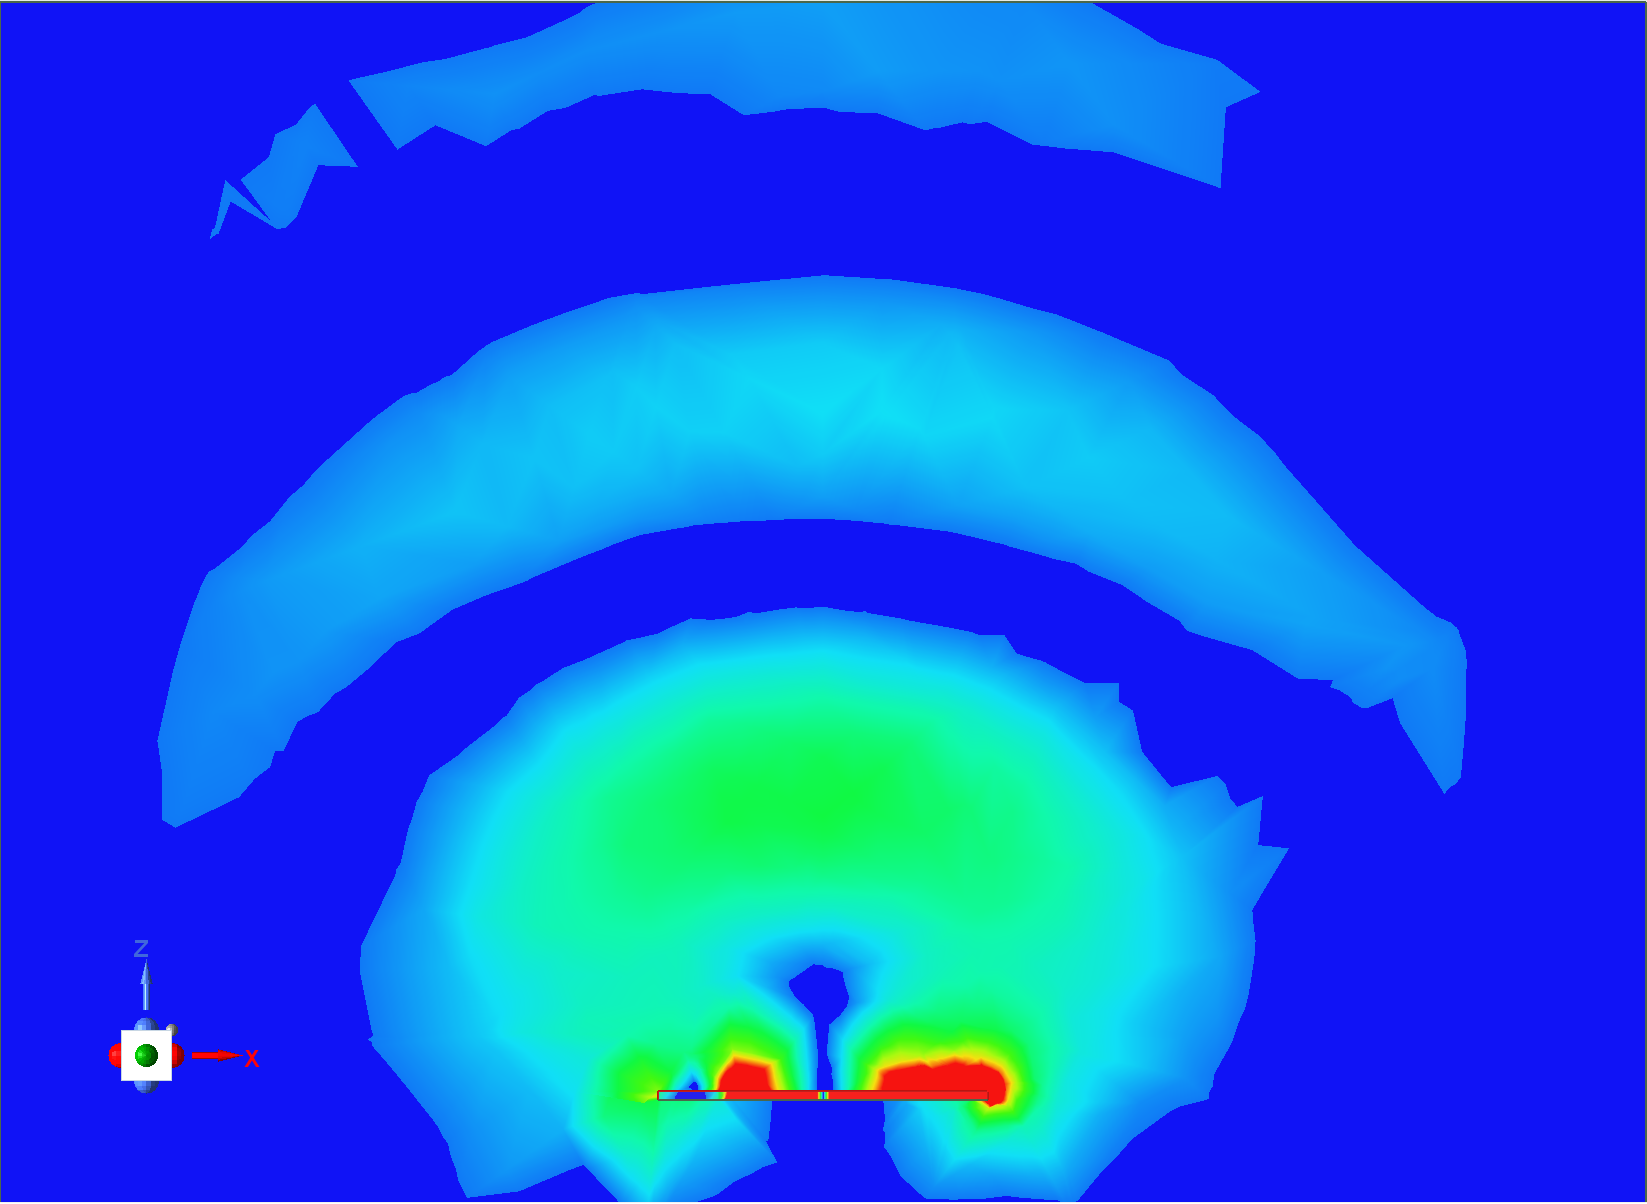
\includegraphics[width=0.35\textwidth]{basic-patch-antenna-radiating-t2.png}
    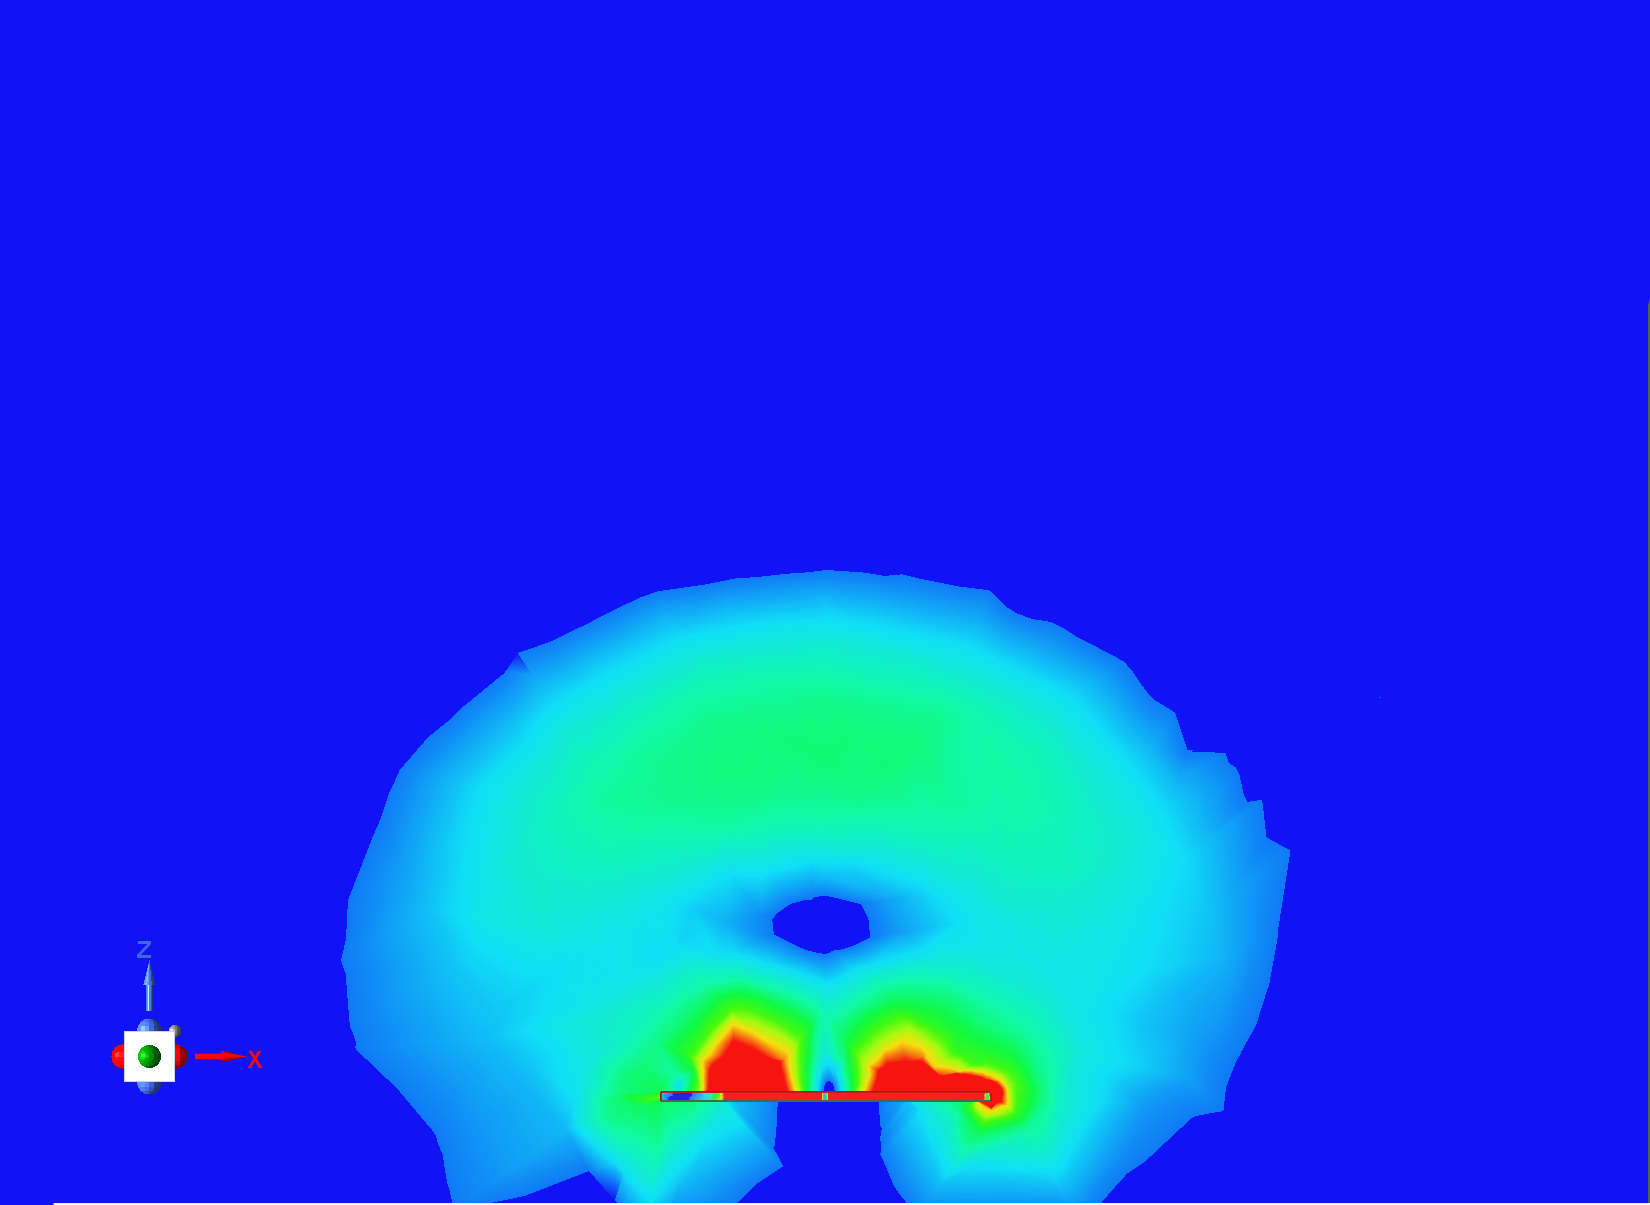
\includegraphics[width=0.35\textwidth]{basic-patch-antenna-radiating-t3.png}
    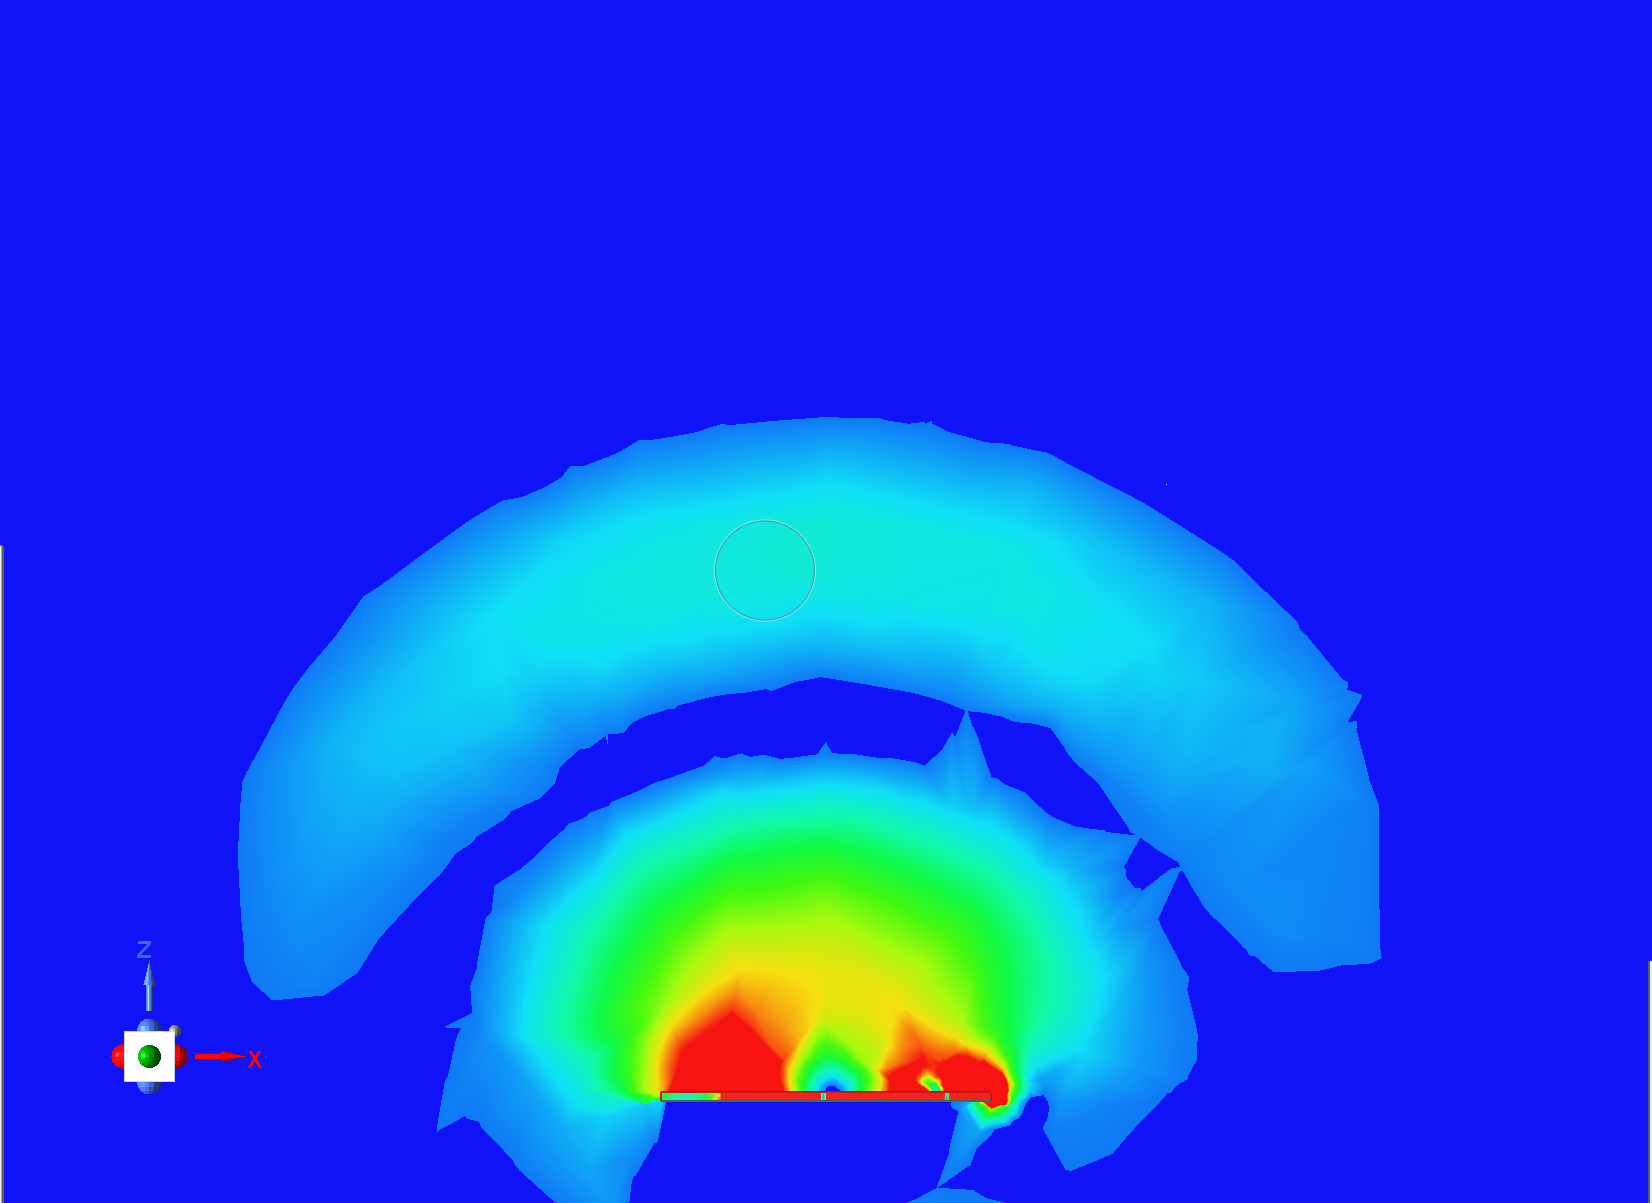
\includegraphics[width=0.35\textwidth]{basic-patch-antenna-radiating-t4.png}
    \caption{The creation of an electromagnetic wave from a patch antenna, at different points in time. The time of each image is from left to right, top to bottom. The bottom image shows a wave detached from the antenna.}
\end{figure} 

\section{Properties}

The simulation shows that patch antennas are broadside radiators, in that they radiate almost all of their energy parallel to the normal of the patch. This leads to patch antennas having a relatively high directivitty. They are generally considered to have moderate gain amongst antennas\cite{khan2015microstrip}. As a result, patch antennas are useful for situations where the positions of the receiver and transmitter are known, so that the antenna may efficiently transmit power to the destination. Alternate use cases include antenna arrays, where the flat profile and high directivitty are very useful, and mobile electronics, due to the flat shape of the antenna. 
\newpage
\begin{figure}[h]
    %\begin{subfigure}{0.5\textwidth}
    \centering
    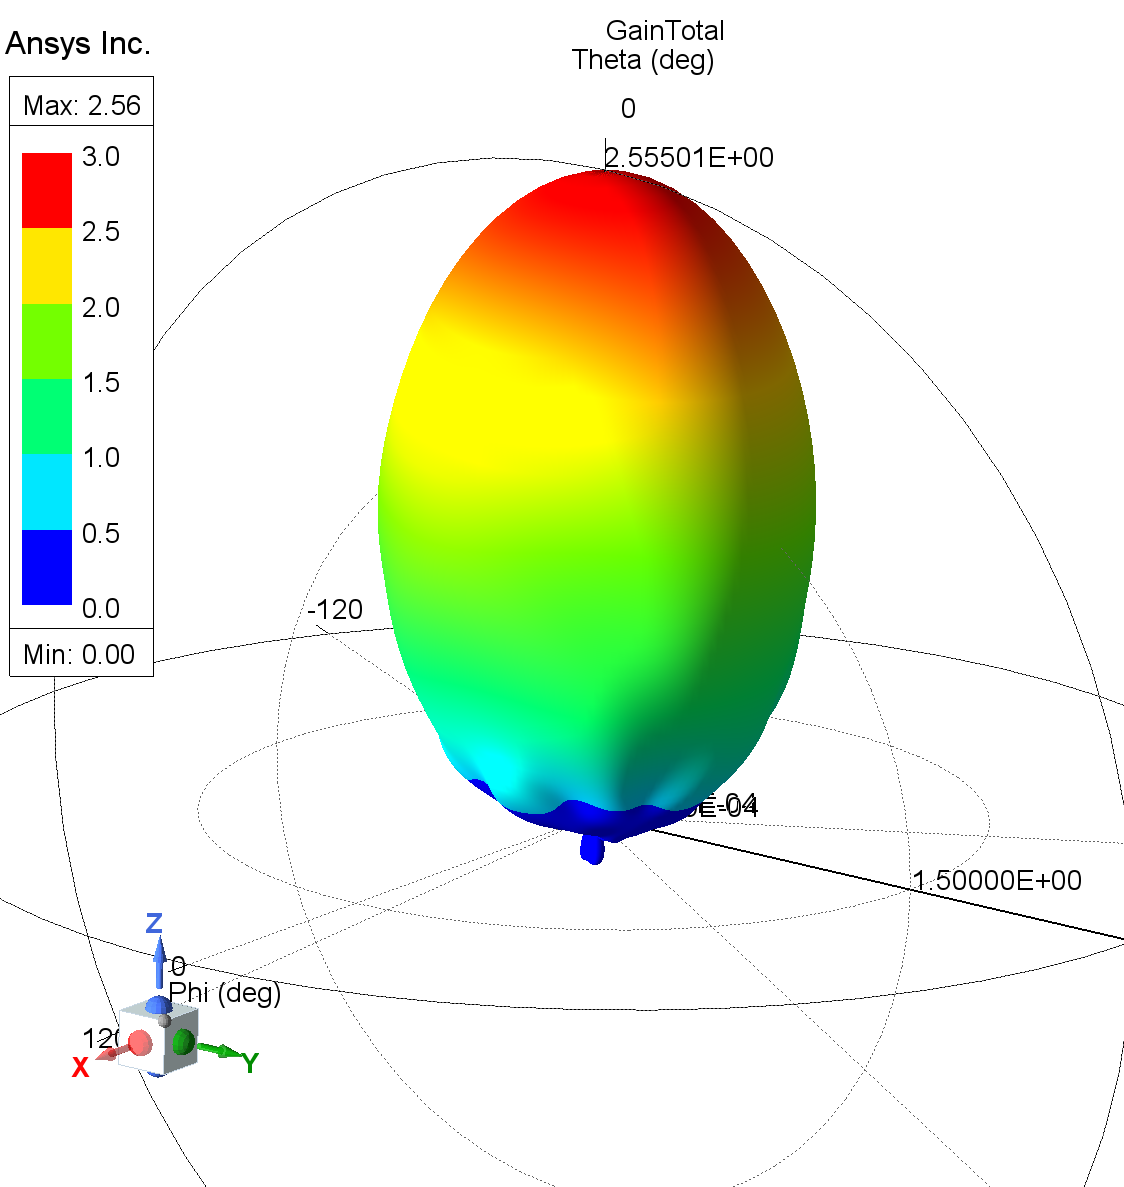
\includegraphics[width=0.45\textwidth]{basic-patch-antenna-gain.png}
    %\end{subfigure}
    \caption{This shows a 3 dimensional polar plot of the gain of the patch antenna described in earlier sections.}
\end{figure}

Besides its high directivitty, the patch antenna presented here has a very narrow bandwidth. Bandwidth refers to the number of frequencies on which the antenna can efficiently radiate power. This is typical for basic patch antennas\cite{balanis2016antenna}. Although having a larger bandwidth is generally preferable in antenna design, some applications, such as military communication, desire antennas with narrow bandwidth\cite{balanis2016antenna}, so the narrow bandwidth is not necessarily undesirable.

\begin{figure}[h]
    %\begin{subfigure}{0.5\textwidth}
    \centering
    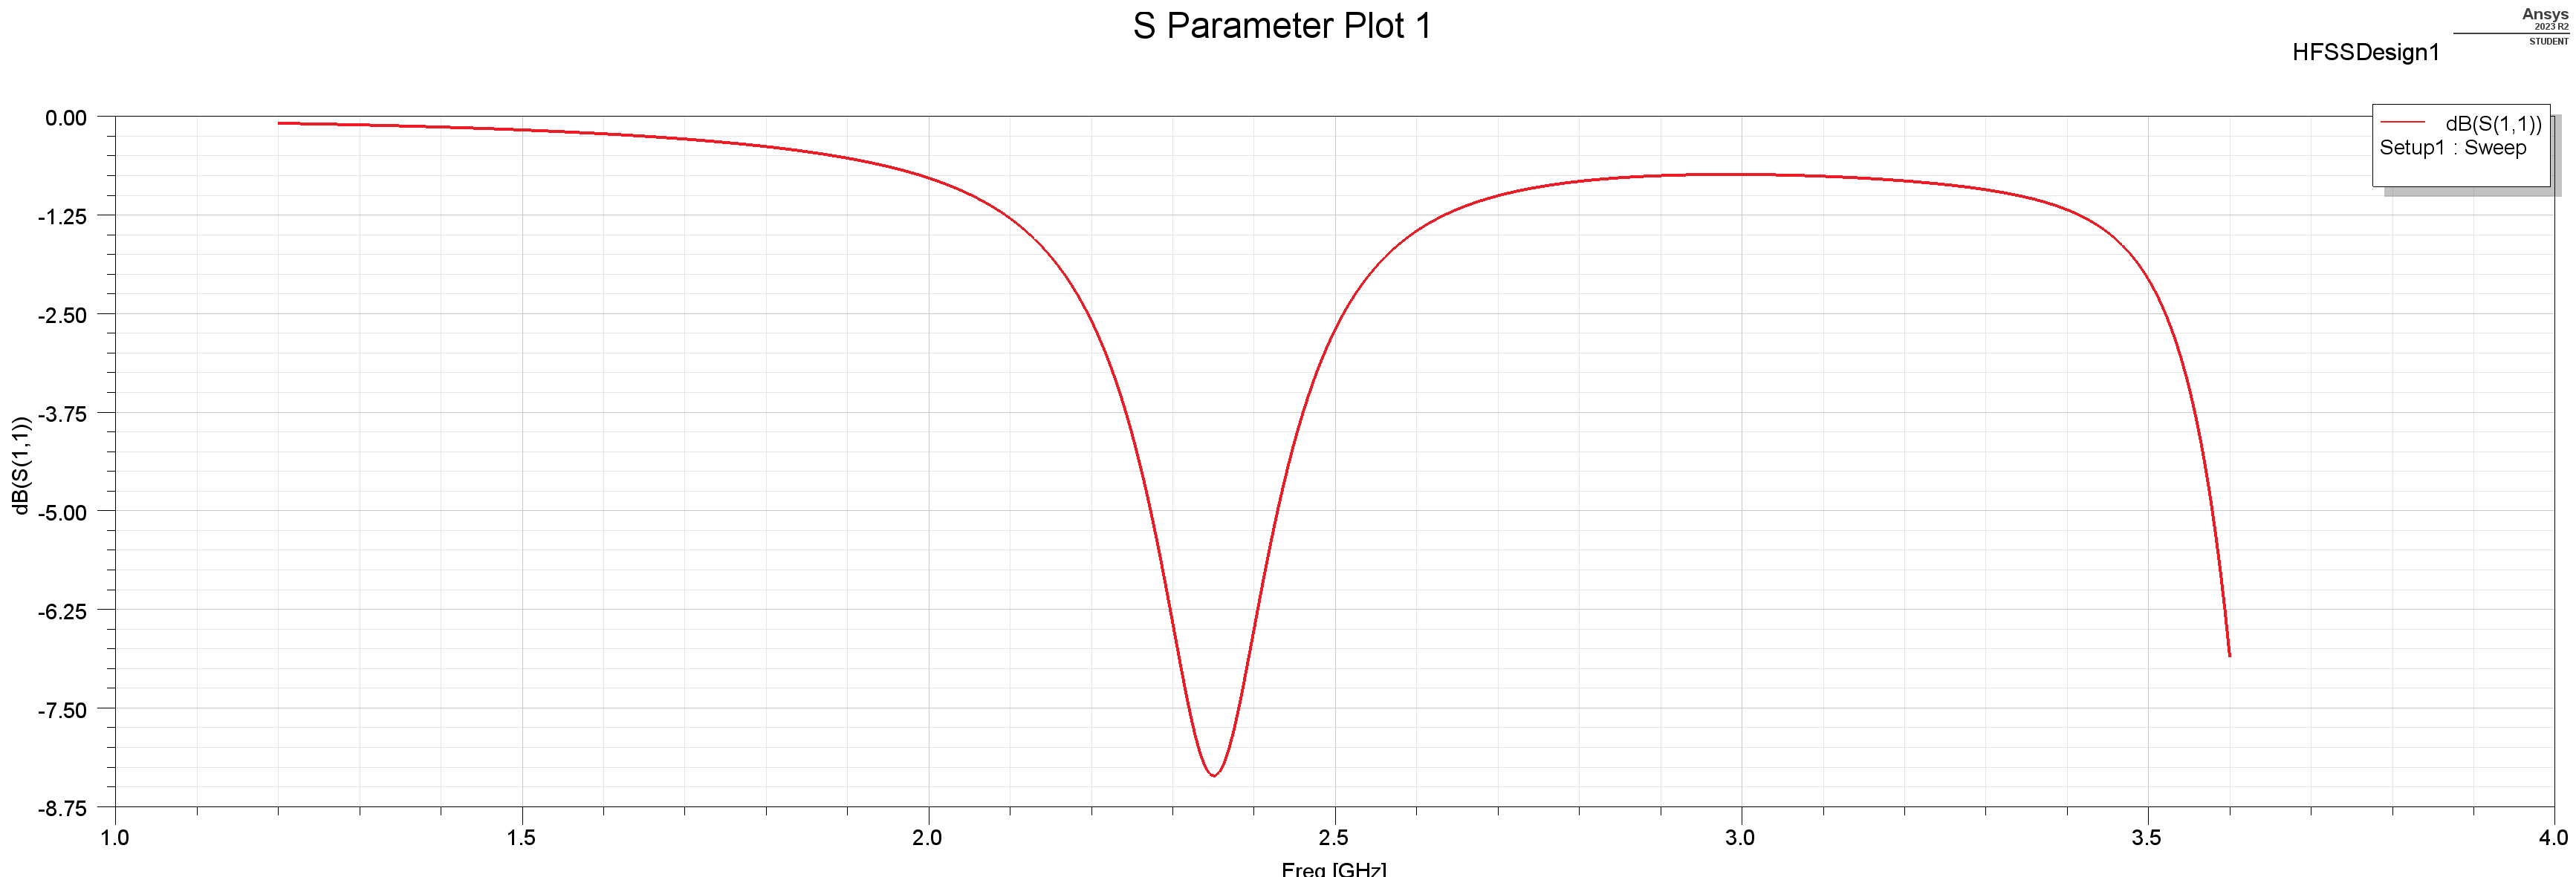
\includegraphics[width=0.9\textwidth]{basic-patch-antenna-splot.png}
    %\end{subfigure}
    \caption{The graph shows the frequency of the signal supplied to the antenna vs the reflection coefficient in decibels. The reflection coefficient of an antenna describes how much of the power being input into an antenna is reflected back to form a standing wave, and thus radiate. A negative reflection coefficient as seen here means that the reflected wave is inverted, which again is necessary for the standing wave to form}
\end{figure}

From figure 11, its clear that this antenna radiates most efficiently at around 2.35 GHz. The narrow bandwidth of the antenna is obvious, due to the narrow valley centered at 2.35 GHz. There is also a drop off towards the far right side of the plot. This is because standing waves can have different resonant modes. The 2.35 GHz frequency happens to be the lowest mode for this antenna design, however, higher modes do also exist.

\section{Conclusion}

Patch antennas are some of the most ubiquitous antennas today, and the body of knowledge accompanying them is vast. This paper gave a mere glimpse into the operation of patch antennas. Although the explanation given for the radiation mechanism for patch antennas given here does adequately explain the operation of a basic rectangular patch antenna, it is insufficient to describe patch antenna radiation as a whole\cite{balanis2016antenna}. Patch antennas have been made with an enormous number of various shapes, and the theory used here would not be able to adequately describe their operation. To address this shortcoming, researchers have worked on other theories to describe patch antenna operation. In addition, much research has been done to overcome the shortcomings of patch antennas, and numerous innovations have been made\cite{balanis2016antenna}. Today, patch antennas can be miniaturized, can be circularly polarized, can have their bandwidth widened, can be used in arrays, and much more. 


\bibliographystyle{IEEEtran}
\bibliography{main}
%\printbibliography


\end{document}
